%%%%%%%%%%%%%%%%%%%%%%%%%%%%%%%%%%%%%%%%%%%%%%%%%%%%%%%%%%%%%%%%%%%%%%%%%%%%%%%%
%                                                                              %
%   2017 -- Diplomamunkavázlat                                                 %
%                                                                              %
%  A latex.feec.vutbr.cz weboldal által szolgáltatott minta alapján készült.   %
%  Importálva azok a csomagok lettek, melyek a mintában is vannak.             %
%                                                                              %
%%%%%%%%%%%%%%%%%%%%%%%%%%%%%%%%%%%%%%%%%%%%%%%%%%%%%%%%%%%%%%%%%%%%%%%%%%%%%%%%
\documentclass[a4paper, 12pt, unicode, czech]{report}
\usepackage[utf8]{inputenc}
\usepackage{graphicx}
\usepackage[nohyperlinks]{acronym}
\usepackage[pdftex,
            pdfauthor={Toth Peter},
            pdftitle={Telemetricky archiv druzic},
            pdfsubject={Semestralni projekt, VUT FEKT UREL, 2017/18},
            pdfkeywords={korekce dopplerskeho posuvu, NO-83, BRICsat, NO-84, PSat, druzice LEO, archiv dat TLE},
            breaklinks=true,
            hypertexnames=false]{hyperref}
\usepackage{pdfpages}
\usepackage{enumitem}
  \setlist{topsep=0pt,partopsep=0pt,noitemsep}
\usepackage{cmap}
\usepackage{upgreek}
\usepackage{dirtree}
\usepackage[formats]{listings}
\lstset{
% Definice jazyka použitého ve výpisech
% language=[LaTeX]{TeX},  % LaTeX
% language={Matlab},      % Matlab
  language={C},           % jazyk C
    basicstyle=\ttfamily, % definice základního stylu písma
    tabsize=2,            % definice velikosti tabulátoru
    inputencoding=utf8,   % pro soubory uložené v kódování UTF-8
    columns=fixed,        % flexible,
    fontadjust=true       % licovani sloupcu
    extendedchars=true,
    literate=             %  definice symbolů s diakritikou
    {á}{{\'a}}1
    {č}{{\v{c}}}1
    {ď}{{\v{d}}}1
    {é}{{\'e}}1
    {ě}{{\v{e}}}1
    {í}{{\'i}}1
    {ň}{{\v{n}}}1
    {ó}{{\'o}}1
    {ř}{{\v{r}}}1
    {š}{{\v{s}}}1
    {ť}{{\v{t}}}1
    {ú}{{\'u}}1
    {ů}{{\r{u}}}1
    {ý}{{\'y}}1
    {ž}{{\v{z}}}1
    {Á}{{\'A}}1
    {Č}{{\v{C}}}1
    {Ď}{{\v{D}}}1
    {É}{{\'E}}1
    {Ě}{{\v{E}}}1
    {Í}{{\'I}}1
    {Ň}{{\v{N}}}1
    {Ó}{{\'O}}1
    {Ř}{{\v{R}}}1
    {Š}{{\v{S}}}1
    {Ť}{{\v{T}}}1
    {Ú}{{\'U}}1
    {Ů}{{\r{U}}}1
    {Ý}{{\'Y}}1
    {Ž}{{\v{Z}}}1
}
\usepackage{nicefrac}   % szép törtek :) -- használata: \nicefrac{a}{b}, ami egy szép a/b formát fog adni
\usepackage{pgfplots}   % DIA-ból exportált ábrákhoz használt csomag használata.
\usepackage{listings}   % Forráskódok szedéséhez alkamazzuk ezt a csomagot.
\usepackage{babel}
\usepackage{lmodern}
\usepackage{textcomp}
\usepackage[T1]{fontenc}

\usepackage[%
%% Z následujících voleb lze použít pouze jednu
% left,               % Rovnice a popisky plovoucich objektů budou %zarovnány vlevo
  center,             % Rovnice a popisky plovoucich objektů budou zarovnány na střed (vychozi)
% Z následujících voleb lze použít pouze jednu
  semestral           % sazba zprávy semestrálního projektu
  %bachelor           % sazba bakalářské práce
  %diploma            % sazba diplomové práce
  %treatise           % sazba pojednání o dizertační práci
  %phd                % sazba dizertační práce
  ]{thesis}           % Balíček pro sazbu studentských prací
                      % Musí být vložen až jako poslední, aby
                      % ostatní balíčky nepřepisovaly jeho příkazy


%%%%%%%%%%%%%%%%%%%%%%%%%%%%%%%%%%%%%%%%%%%%%%%%%%%%%%%%%%%%%%%%%%%%%%%%%%%%%%%%
%                                                                              %
%   Paraméterek külső állományból való betöltése.                              %
%                                                                              %
%%%%%%%%%%%%%%%%%%%%%%%%%%%%%%%%%%%%%%%%%%%%%%%%%%%%%%%%%%%%%%%%%%%%%%%%%%%%%%%%
\autor[Bc.]{Péter}{Tóth}
\vedouci[Ing.]{Tomáš}{Urbanec }[Ph.D.]
\nazev{Telemetrický archiv družic}{Satellite telemetry archive}
%\oponent[doc.\ Mgr.]{Křestní}{Příjmení}[Ph.D.]
\oborstudia{Radioelektronika}{Radioelectronics}
\fakulta{Fakulta elektrotechniky a komunikačních technologií}{Faculty of Electrical Engineering and Communication}
\ustav{Ústav radioelektroniky}{Department of Radio Electronics}
\logofakulta{loga/FEKT_zkratka_barevne_PANTONE_CZ}
\rok{2017}
\datum{19.\,12.\,2017} % Datum se uplatní pouze v prezentaci k obhajobě
\misto{Brno}
\abstrakt{Táto práce se zaobírá zpracováním přijatých signálů z amatérských družic NO-83 a NO-84 ParkinsonSat na nízké oběžné dráze (Low Earth Orbit – LEO) vysílajících telemetrické údaje v pásmu $70\,\mathrm{cm}$ vln. které jsou postiženy dopplerovským posuvem kmitočtu. Kvůli povaze oběžné dráhy a kmitočtu vysílání, přijatý signál je znatelně poškozen dopplerovským posuvem kmitočtu, který se musí kompenzovat pro pozdější potřeby demodulace.
}{This project work is dealing with processing of received radio signals of LEO satellites NO-83 and NO-84 ParkinsonSat transmitting in the 70--centimeter band. The nature of this kind of setup makes the received signal bearing a large amount of Doppler shift, which needs to be compensated in order to demodulate it.
}
\klicovaslova{korekce dopplerského posuvu, NO-83, BRICsat, NO-84, PSat, družice LEO, archiv dat TLE}
  {doppler shift correction, NO-83, BRICsat, NO-84, PSat, LEO satellites, TLE data archive}
\podekovanitext{Rád bych poděkoval vedoucímu diplomové práce panu Ing.~Tomášu Urbanci, Ph.D.\ za odborné vedení, konzultace, trpělivost a podnětné návrhy k~práci.}




%%%%%%%%%%%%%%%%%%%%%%%%%%%%%%%%%%%%%%%%%%%%%%%%%%%%%%%%%%%%%%%%%%%%%%%%%%%%%%%%
%                                                                              %
%   A diplomamunka vázlat szöveges részének kezdete.                           %
%                                                                              %
%%%%%%%%%%%%%%%%%%%%%%%%%%%%%%%%%%%%%%%%%%%%%%%%%%%%%%%%%%%%%%%%%%%%%%%%%%%%%%%%
\begin{document}
  \includepdf[pages=1,offset=15.4mm -1in]{pdf/desky_xtothp00.pdf}     % Vložení desek generovaných informačním systémem
  \setcounter{page}{1}                                                % Resetovani citace stranek - desky se necisluji
  \includepdf[pages=1,offset=15.4mm -1in]{pdf/titulni_list_cb.pdf}    % Vložení titulního listu generovaného informačním systémem
  \includepdf[pages=1,offset=15.4mm -1in]{pdf/zadani_xtothp00_cb.pdf} % Vložení zadání generovaného informačním systémem

%%%%%%%%%%%%%%%%%%%%%%%%%%%%%%%%%%%%%%%%%%%%%%%%%%%%%%%%%%%%%%%%%%%%%%%%%%%%%%%%
% A tartalmi kivonat, köszönet rész.
  \vytvorabstrakt
  \vytvorprohlaseni
  \vytvorpodekovani

%%%%%%%%%%%%%%%%%%%%%%%%%%%%%%%%%%%%%%%%%%%%%%%%%%%%%%%%%%%%%%%%%%%%%%%%%%%%%%%%
% A tartalmak, felsorolások része.
  \obsah
  \seznamobrazku
  \seznamtabulek
  \lstlistoflistings

%%%%%%%%%%%%%%%%%%%%%%%%%%%%%%%%%%%%%%%%%%%%%%%%%%%%%%%%%%%%%%%%%%%%%%%%%%%%%%%%
% Az érdemi szöveg itt kezdődik.
  \chapter*{Úvod}
\phantomsection
\addcontentsline{toc}{chapter}{Úvod}

Radiokomunikace prošla ohromným vývojem v průběhu druhé polovice 20. století. Vypuštění první umělé družice Sputnik-1 v roce 1957 datujeme začátek vesmírného věku. Od té doby se otevřeli nové možnosti radioamatérův věnovat se svému koníčku, nebo výzkumu.

Necelé čtyři roky po vypuštění první umělé družice Země se svět dočkal první amatérské umělé družice sestrojeného v rámci projektu \zkratka{OSCAR} \cite{wiki:amateur_sat}, kterého nástupnickou organizaci se stal \zkratka{AMSAT} \cite{wiki:AMSAT}. Družice OSCAR I byla vypuštěná na nízkou oběžnou dráhu jako druhotný náklad, který vyžíval rezervy nosnosti rakety  Thor DM-21 Agena-B. Tento způsob dopravy byl zvolen z ekonomických důvodů a je dodnes používán.

Obecně se amatérské družice nasazují na nízkou oběžnou dráhu (Low Earth Orbit -- LEO) \cite{book:ARRL_handbook}. Výhodou dráhy tohoto typu je jejich finanční nenáročnost, co je zčásti způsobená vlastností plynoucího z nazvu oběžné dráhy, výškou orbitu, který se pohybuje od $300\,\mathrm{km}$ do $2000\,\mathrm{km}$. Nedostatkem nízké oběžné dráhy je vysoká relativní rychlost družice vůči pozemní stanici, která přibližně $7{,}8\,\mathrm{\nicefrac{km}{s}}$ \cite{wiki:LEO} jehož důsledkem je rádiový signál značně postižen dopplerovským posuvem kmitočtu, kterého velikost dosahuje i $26\,\mathrm{ppm}$.

\section*{Cíle práce}
\phantomsection
\addcontentsline{toc}{section}{Cíle práce}
Na palubě družic se nacházejí přístroje určené k měření elektrických i neelektrických veličin charakterizující stav kosmické lodi. Tyto údaje jsou v jistých časových okamžicích odvysílané směrem na Zem.

Cílem této práce je zpracování přijatého signálu postiženého dopplerovským posuvem, demodulace a dekódování signálu a následná archivace dat pro její budoucí analyzování .

  \chapter[Struční přehled amaterských družic]{Struční přehled\\ amaterských družic}

Radiokomunikace prošla ohromným vývojem v průběhu druhé polovice 20. století. Vypuštění první umělé družice Sputnik-1 v roce 1957 datujeme začátek vesmírného věku. Od té doby se otevřeli nové možnosti radioamatérův věnovat se svému koníčku, nebo výzkumu.

    Necelé čtyři roky po vypuštění první umělé družice Země se svět dočkal první amatérské umělé družice sestrojeného v rámci projektu \zkratka{OSCAR} \cite{wiki:amateur_sat}, kterého nástupnickou organizaci se stal \zkratka{AMSAT} \cite{wiki:AMSAT}. Družice OSCAR I byla vypuštěná na nízkou oběžnou dráhu jako druhotný náklad, který vyžíval rezervy nosnosti rakety  Thor DM-21 Agena-B. Tento způsob dopravy byl zvolen z ekonomických důvodů a je dodnes používán.

    Obecně se amatérské družice nasazují na nízkou oběžnou dráhu (Low Earth Orbit -- LEO) \cite{book:ARRL_handbook}. Výhodou dráhy tohoto typu je jejich finanční nenáročnost, co je zčásti způsobená vlastností plynoucího z nazvu oběžné dráhy, výškou orbitu, který se pohybuje od $300\,\mathrm{km}$ do $2000\,\mathrm{km}$. Nedostatkem nízké oběžné dráhy je vysoká relativní rychlost družice vůči pozemní stanici, která přibližně $7{,}8\,\mathrm{\nicefrac{km}{s}}$ \cite{wiki:LEO} jehož důsledkem je rádiový signál značně postižen dopplerovským posuvem kmitočtu, kterého velikost dosahuje i $26\,\mathrm{ppm}$.



\chapter{Sledování a predikce pohybu těles na oběžné dráze Země}

Objekty, které se pohybují vesmírem kolem Země jsou sledovány organizacemi \cite{wiki:derbis}:
\begin{itemize}
    \item \zkratka{USSTRATCOM}(součást \zkratka{DoD})
    \item \zkratka{ESA}
    \item \zkratka{Fraunhofer-FHR}
    \item \zkratka{JPL}(součast \zkratka{NASA})
    \item \zkratka{MIT}
    \item \zkratka{EISCAT}
    \item \zkratka{USAF}
\end{itemize}

Ke sledování se používají pozemní radary, lidary, pozemní  a vesmírné teleskopy. Mezi sledované objekty patří umělé družice, pozůstatky raket a jiný vesmírný odpad. Nejrozsáhlejší katalog stavu družic udržuje Ministerstvo obrany Spojených států (\zkratka{DoD}) s názvem Space Object Catalog. Civilní varianta této databáze je provozována organizaci \zkratka{NASA}. Tyto databáze se udržují pomocí různých modelů orbitální mechaniky. Pohyby družic jsou analyticky vypočteny pomocí teorie všeobecných perturbací. Prvky dráhy této teorie jsou publikovány ve formátu \zkratka{NASA}/NORAD \zkratka{TLE}. \cite{wiki:US_space_surv}.

Proč se zabývat přesnou polohou družice? Aby jsme byly schopní provést korekci dopplerovského posuvu, musíme splnit několik požadavek výpočtu:
\begin{itemize}
%  \item přesný čas
  \item polohu pozemní stanice \footnote{pozemní stanici považujeme za stacionární vzhledem ke povrchu Země}
  \item polohu a rychlost umělé družice
\end{itemize}

%Pro korekci dopplerovského posuvu frekvence musíme znát polohu naši pozemní stanice, polohu družice a předpovědět její polohu. K tomu pozdějšímu nám právě napomáhají prvky dráhy ze souborů \zkratka{TLE} využívajíc model \zkratka{SGP4} \cite{wiki:TLE}.

\chapter{Výpočet rychlosti těles na oběžní dráze Země}
  TBD\dots

\chapter{Určení dopplerovského posuvu}
  TBD\dots

\chapter{Korekce dopplerovského posuvu}
  TBD\dots

\chapter{Demodulace a dekódování signálu}
  TBD\dots

  \chapter[Realizace skriptů v jazyce Python 3]{Realizace skriptů\\ v jazyce Python 3}
\label{chap:python3}

\section{Vytvoření archivu dat TLE}
  Vytvoření lokální databázi dat TLE je nezbytné pro správnou korekci dopplerovského posuvu. Pro umělé družice NO-83 a NO-84 jsou veřejně přístupné data TLE na stránce organizace \zkratka{AMSAT}: <\url{http://amsat.org/pipermail/keps/}>. Tyto data jsou distribuované formou elektronického mailing list, kterého archív se nachází na výše zmíněném URL v jedním souboru. Aby bylo možné použit údaje TLE obsáhnuty v tomhle archivním souboru, je nutné provést extrakci dat TLE dle datu jejího vzniku.

  Na obrázku \ref{fig:TLE_flow} je uveden vývojový diagram skriptu pro extrahování dat TLE. Jako povinný vstupní parametr je název souboru staženého z webové stránky oragnizace \zkratka{AMSAT}. Data TLE jsou posílané v jednom emailu. Skript identifikuje začátek i konec balíků dat TLE. Na začátku každého balíku se hledjí vzory:\\
  \texttt{SB\textbackslash s+KEPS\textbackslash s+@\textbackslash s+AMSAT\textbackslash s+\$ORB\textbackslash d{5}\textbackslash.[A-Z]}\\
  \texttt{\textasciicircum 2Line}\\
  pomocí nástroje na vyhledávání regulárních výrazů implementovaného modulem re ze standardní knihovny jazyka Python. Konec bálíka je značen řetězcem
  \texttt{\textbackslash EX}.

  V případě, že skript narazí na hledaný výraz, nastaví se příslušný příznak. Tyto příznaky zaručí, aby řádky jednoho balíku se připojili k jednomu řetězci. Když skript identifikuje poslední řádek, pospojovaný řetězec řádků se připojí k množině všech balíků TLE dat. Návratovou hodnotou je právě tato množina. Množina v jazyce Python 3 zaručuje jedinečnost všech prvků, obdobně jako množiny z teorie množin.

  K výpisu souboru patří funkce \texttt{dump\_to\_file} skriptu \texttt{TLE.py}. Tato funkce má jeden povinný parametr, množinu dat TLE. Z této množiny se načte každý jeden prvek. V těchto prvcích se prohledává datum vzniku, což se použije jako název souboru. Následně se dle potřeby vytvoří adresář, kterého název je rok vzniku TLE dat. Před vytvářením adresáře se kontroluje přítomnost adresáře, nebo souboru stejného jména, jaký se chystá být vytvořit. Jestli adresář se stejným jménem existuje, začne se de ní zapisovat. V opačném případě předpokládáme, že v adresáři je soubor se stejný jménem musíme název složky, kterou se chystáme vytvořit změnit z důvodu nemožnosti koexistence souboru a adresáře stejného jména v rodičovském adresáři. K názvu složky se přidává znak podtržítka a číslo, které se iteruje inkrementací do doby, kdy v rodičovském se nebude nacházet soubor se stejným jménem. V případě adresáře se stejným jménem nalezeného po přidání dodatečných znaků k názvu souboru, se adresář začne používat k uložení souborů. Čtení z množiny je realizováno pomocí iterací nad její prvkami.

%  % Graphic for TeX using PGF
% Title: /home/ptoth/Documents/Projekt/github/projekt17/LaTeX/obrazky/TLE.bb
% Creator: Dia v0.97.3
% CreationDate: Sun Dec 10 19:15:52 2017
% For: ptoth
% \usepackage{tikz}
% The following commands are not supported in PSTricks at present
% We define them conditionally, so when they are implemented,
% this pgf file will use them.
\ifx\du\undefined
  \newlength{\du}
\fi
\setlength{\du}{15\unitlength}
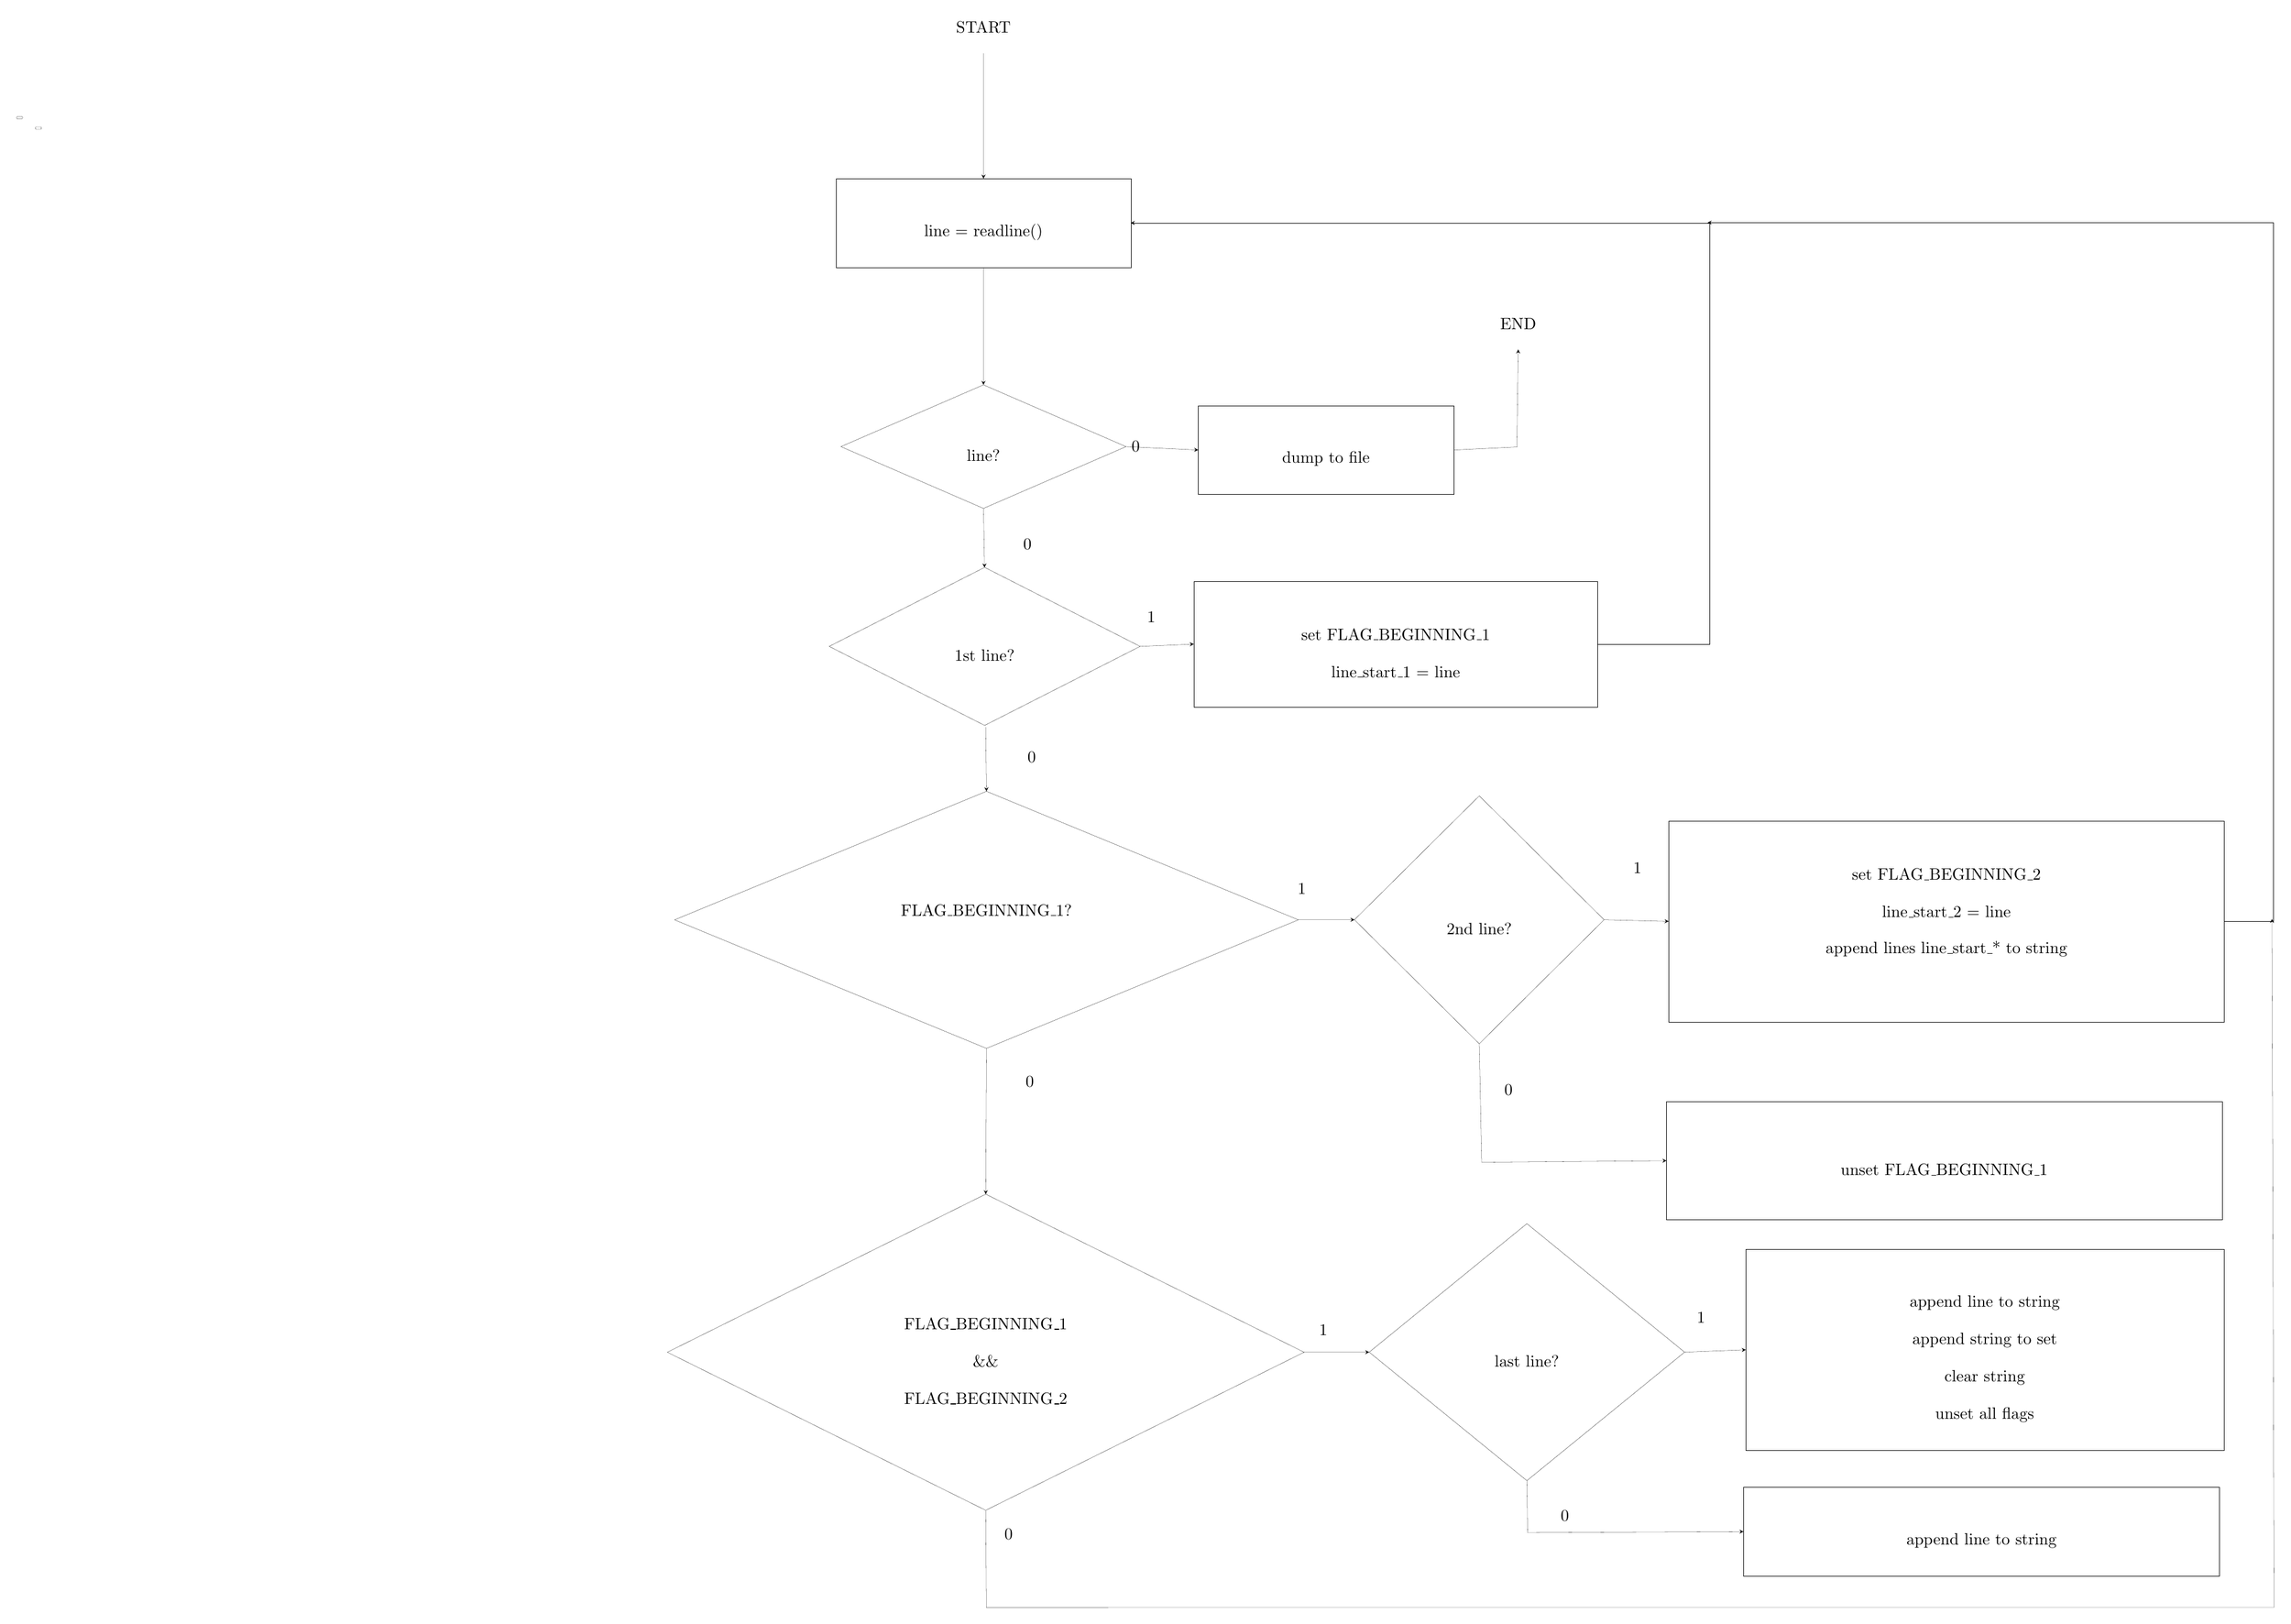
\begin{tikzpicture}
\pgftransformxscale{1.000000}
\pgftransformyscale{-1.000000}
\definecolor{dialinecolor}{rgb}{0.000000, 0.000000, 0.000000}
\pgfsetstrokecolor{dialinecolor}
\definecolor{dialinecolor}{rgb}{1.000000, 1.000000, 1.000000}
\pgfsetfillcolor{dialinecolor}
\pgfsetlinewidth{0.100000\du}
\pgfsetdash{}{0pt}
\pgfsetdash{}{0pt}
\pgfsetbuttcap
\pgfsetmiterjoin
\pgfsetlinewidth{0.100000\du}
\pgfsetbuttcap
\pgfsetmiterjoin
\pgfsetdash{}{0pt}
\definecolor{dialinecolor}{rgb}{1.000000, 1.000000, 1.000000}
\pgfsetfillcolor{dialinecolor}
\pgfpathmoveto{\pgfpoint{20.120130\du}{-2.961170\du}}
\pgfpathlineto{\pgfpoint{22.640951\du}{-2.961170\du}}
\pgfpathcurveto{\pgfpoint{22.989004\du}{-2.961170\du}}{\pgfpoint{23.271156\du}{-2.624692\du}}{\pgfpoint{23.271156\du}{-2.209625\du}}
\pgfpathcurveto{\pgfpoint{23.271156\du}{-1.794557\du}}{\pgfpoint{22.989004\du}{-1.458079\du}}{\pgfpoint{22.640951\du}{-1.458079\du}}
\pgfpathlineto{\pgfpoint{20.120130\du}{-1.458079\du}}
\pgfpathcurveto{\pgfpoint{19.772077\du}{-1.458079\du}}{\pgfpoint{19.489924\du}{-1.794557\du}}{\pgfpoint{19.489924\du}{-2.209625\du}}
\pgfpathcurveto{\pgfpoint{19.489924\du}{-2.624692\du}}{\pgfpoint{19.772077\du}{-2.961170\du}}{\pgfpoint{20.120130\du}{-2.961170\du}}
\pgfusepath{fill}
\definecolor{dialinecolor}{rgb}{0.000000, 0.000000, 0.000000}
\pgfsetstrokecolor{dialinecolor}
\pgfpathmoveto{\pgfpoint{20.120130\du}{-2.961170\du}}
\pgfpathlineto{\pgfpoint{22.640951\du}{-2.961170\du}}
\pgfpathcurveto{\pgfpoint{22.989004\du}{-2.961170\du}}{\pgfpoint{23.271156\du}{-2.624692\du}}{\pgfpoint{23.271156\du}{-2.209625\du}}
\pgfpathcurveto{\pgfpoint{23.271156\du}{-1.794557\du}}{\pgfpoint{22.989004\du}{-1.458079\du}}{\pgfpoint{22.640951\du}{-1.458079\du}}
\pgfpathlineto{\pgfpoint{20.120130\du}{-1.458079\du}}
\pgfpathcurveto{\pgfpoint{19.772077\du}{-1.458079\du}}{\pgfpoint{19.489924\du}{-1.794557\du}}{\pgfpoint{19.489924\du}{-2.209625\du}}
\pgfpathcurveto{\pgfpoint{19.489924\du}{-2.624692\du}}{\pgfpoint{19.772077\du}{-2.961170\du}}{\pgfpoint{20.120130\du}{-2.961170\du}}
\pgfusepath{stroke}
% setfont left to latex
\definecolor{dialinecolor}{rgb}{0.000000, 0.000000, 0.000000}
\pgfsetstrokecolor{dialinecolor}
\node at (21.380540\du,-2.009625\du){START};
\pgfsetlinewidth{0.100000\du}
\pgfsetdash{}{0pt}
\pgfsetdash{}{0pt}
\pgfsetbuttcap
{
\definecolor{dialinecolor}{rgb}{0.000000, 0.000000, 0.000000}
\pgfsetfillcolor{dialinecolor}
% was here!!!
\pgfsetarrowsend{stealth}
\definecolor{dialinecolor}{rgb}{0.000000, 0.000000, 0.000000}
\pgfsetstrokecolor{dialinecolor}
\draw (21.380540\du,-1.458079\du)--(21.381739\du,1.225647\du);
}
\definecolor{dialinecolor}{rgb}{1.000000, 1.000000, 1.000000}
\pgfsetfillcolor{dialinecolor}
\fill (21.381071\du,5.642039\du)--(24.432535\du,6.964810\du)--(21.381071\du,8.287581\du)--(18.329607\du,6.964810\du)--cycle;
\pgfsetlinewidth{0.100000\du}
\pgfsetdash{}{0pt}
\pgfsetdash{}{0pt}
\pgfsetmiterjoin
\definecolor{dialinecolor}{rgb}{0.000000, 0.000000, 0.000000}
\pgfsetstrokecolor{dialinecolor}
\draw (21.381071\du,5.642039\du)--(24.432535\du,6.964810\du)--(21.381071\du,8.287581\du)--(18.329607\du,6.964810\du)--cycle;
% setfont left to latex
\definecolor{dialinecolor}{rgb}{0.000000, 0.000000, 0.000000}
\pgfsetstrokecolor{dialinecolor}
\node at (21.381071\du,7.159810\du){line?};
\pgfsetlinewidth{0.100000\du}
\pgfsetdash{}{0pt}
\pgfsetdash{}{0pt}
\pgfsetbuttcap
{
\definecolor{dialinecolor}{rgb}{0.000000, 0.000000, 0.000000}
\pgfsetfillcolor{dialinecolor}
% was here!!!
\pgfsetarrowsend{stealth}
\definecolor{dialinecolor}{rgb}{0.000000, 0.000000, 0.000000}
\pgfsetstrokecolor{dialinecolor}
\draw (21.381739\du,3.125647\du)--(21.381071\du,5.642039\du);
}
\definecolor{dialinecolor}{rgb}{1.000000, 1.000000, 1.000000}
\pgfsetfillcolor{dialinecolor}
\fill (18.230355\du,1.225647\du)--(18.230355\du,3.125647\du)--(24.533123\du,3.125647\du)--(24.533123\du,1.225647\du)--cycle;
\pgfsetlinewidth{0.100000\du}
\pgfsetdash{}{0pt}
\pgfsetdash{}{0pt}
\pgfsetmiterjoin
\definecolor{dialinecolor}{rgb}{0.000000, 0.000000, 0.000000}
\pgfsetstrokecolor{dialinecolor}
\draw (18.230355\du,1.225647\du)--(18.230355\du,3.125647\du)--(24.533123\du,3.125647\du)--(24.533123\du,1.225647\du)--cycle;
% setfont left to latex
\definecolor{dialinecolor}{rgb}{0.000000, 0.000000, 0.000000}
\pgfsetstrokecolor{dialinecolor}
\node at (21.381739\du,2.370647\du){line = readline()};
% setfont left to latex
\definecolor{dialinecolor}{rgb}{0.000000, 0.000000, 0.000000}
\pgfsetstrokecolor{dialinecolor}
\node[anchor=west] at (24.432535\du,6.964810\du){0};
\definecolor{dialinecolor}{rgb}{1.000000, 1.000000, 1.000000}
\pgfsetfillcolor{dialinecolor}
\fill (25.976934\du,6.086417\du)--(25.976934\du,7.986417\du)--(31.447244\du,7.986417\du)--(31.447244\du,6.086417\du)--cycle;
\pgfsetlinewidth{0.100000\du}
\pgfsetdash{}{0pt}
\pgfsetdash{}{0pt}
\pgfsetmiterjoin
\definecolor{dialinecolor}{rgb}{0.000000, 0.000000, 0.000000}
\pgfsetstrokecolor{dialinecolor}
\draw (25.976934\du,6.086417\du)--(25.976934\du,7.986417\du)--(31.447244\du,7.986417\du)--(31.447244\du,6.086417\du)--cycle;
% setfont left to latex
\definecolor{dialinecolor}{rgb}{0.000000, 0.000000, 0.000000}
\pgfsetstrokecolor{dialinecolor}
\node at (28.712089\du,7.231417\du){dump to file};
\pgfsetlinewidth{0.100000\du}
\pgfsetdash{}{0pt}
\pgfsetdash{}{0pt}
\pgfsetbuttcap
{
\definecolor{dialinecolor}{rgb}{0.000000, 0.000000, 0.000000}
\pgfsetfillcolor{dialinecolor}
% was here!!!
\pgfsetarrowsend{stealth}
\definecolor{dialinecolor}{rgb}{0.000000, 0.000000, 0.000000}
\pgfsetstrokecolor{dialinecolor}
\draw (24.432535\du,6.964810\du)--(25.976934\du,7.036417\du);
}
\definecolor{dialinecolor}{rgb}{1.000000, 1.000000, 1.000000}
\pgfsetfillcolor{dialinecolor}
\fill (21.406367\du,9.549864\du)--(24.733658\du,11.242064\du)--(21.406367\du,12.934265\du)--(18.079077\du,11.242064\du)--cycle;
\pgfsetlinewidth{0.100000\du}
\pgfsetdash{}{0pt}
\pgfsetdash{}{0pt}
\pgfsetmiterjoin
\definecolor{dialinecolor}{rgb}{0.000000, 0.000000, 0.000000}
\pgfsetstrokecolor{dialinecolor}
\draw (21.406367\du,9.549864\du)--(24.733658\du,11.242064\du)--(21.406367\du,12.934265\du)--(18.079077\du,11.242064\du)--cycle;
% setfont left to latex
\definecolor{dialinecolor}{rgb}{0.000000, 0.000000, 0.000000}
\pgfsetstrokecolor{dialinecolor}
\node at (21.406367\du,11.437064\du){1st line?};
\pgfsetlinewidth{0.100000\du}
\pgfsetdash{}{0pt}
\pgfsetdash{}{0pt}
\pgfsetbuttcap
{
\definecolor{dialinecolor}{rgb}{0.000000, 0.000000, 0.000000}
\pgfsetfillcolor{dialinecolor}
% was here!!!
\pgfsetarrowsend{stealth}
\definecolor{dialinecolor}{rgb}{0.000000, 0.000000, 0.000000}
\pgfsetstrokecolor{dialinecolor}
\draw (21.381071\du,8.287581\du)--(21.403561\du,9.551439\du);
}
\definecolor{dialinecolor}{rgb}{1.000000, 1.000000, 1.000000}
\pgfsetfillcolor{dialinecolor}
\fill (25.882086\du,9.843397\du)--(25.882086\du,12.543397\du)--(34.527086\du,12.543397\du)--(34.527086\du,9.843397\du)--cycle;
\pgfsetlinewidth{0.100000\du}
\pgfsetdash{}{0pt}
\pgfsetdash{}{0pt}
\pgfsetmiterjoin
\definecolor{dialinecolor}{rgb}{0.000000, 0.000000, 0.000000}
\pgfsetstrokecolor{dialinecolor}
\draw (25.882086\du,9.843397\du)--(25.882086\du,12.543397\du)--(34.527086\du,12.543397\du)--(34.527086\du,9.843397\du)--cycle;
% setfont left to latex
\definecolor{dialinecolor}{rgb}{0.000000, 0.000000, 0.000000}
\pgfsetstrokecolor{dialinecolor}
\node at (30.204586\du,10.988397\du){set FLAG\_BEGINNING\_1};
% setfont left to latex
\definecolor{dialinecolor}{rgb}{0.000000, 0.000000, 0.000000}
\pgfsetstrokecolor{dialinecolor}
\node at (30.204586\du,11.788397\du){line\_start\_1 = line};
\pgfsetlinewidth{0.100000\du}
\pgfsetdash{}{0pt}
\pgfsetdash{}{0pt}
\pgfsetbuttcap
{
\definecolor{dialinecolor}{rgb}{0.000000, 0.000000, 0.000000}
\pgfsetfillcolor{dialinecolor}
% was here!!!
\pgfsetarrowsend{stealth}
\definecolor{dialinecolor}{rgb}{0.000000, 0.000000, 0.000000}
\pgfsetstrokecolor{dialinecolor}
\draw (24.733658\du,11.242064\du)--(25.882086\du,11.193397\du);
}
% setfont left to latex
\definecolor{dialinecolor}{rgb}{0.000000, 0.000000, 0.000000}
\pgfsetstrokecolor{dialinecolor}
\node[anchor=west] at (24.765215\du,10.614032\du){1};
\pgfsetlinewidth{0.100000\du}
\pgfsetdash{}{0pt}
\pgfsetdash{}{0pt}
\pgfsetmiterjoin
\pgfsetbuttcap
{
\definecolor{dialinecolor}{rgb}{0.000000, 0.000000, 0.000000}
\pgfsetfillcolor{dialinecolor}
% was here!!!
\pgfsetarrowsend{stealth}
{\pgfsetcornersarced{\pgfpoint{0.000000\du}{0.000000\du}}\definecolor{dialinecolor}{rgb}{0.000000, 0.000000, 0.000000}
\pgfsetstrokecolor{dialinecolor}
\draw (34.527086\du,11.193397\du)--(36.917283\du,11.193397\du)--(36.917283\du,2.175647\du)--(24.533123\du,2.175647\du);
}}
\definecolor{dialinecolor}{rgb}{1.000000, 1.000000, 1.000000}
\pgfsetfillcolor{dialinecolor}
\fill (21.445061\du,14.344899\du)--(28.120138\du,17.097124\du)--(21.445061\du,19.849349\du)--(14.769983\du,17.097124\du)--cycle;
\pgfsetlinewidth{0.100000\du}
\pgfsetdash{}{0pt}
\pgfsetdash{}{0pt}
\pgfsetmiterjoin
\definecolor{dialinecolor}{rgb}{0.000000, 0.000000, 0.000000}
\pgfsetstrokecolor{dialinecolor}
\draw (21.445061\du,14.344899\du)--(28.120138\du,17.097124\du)--(21.445061\du,19.849349\du)--(14.769983\du,17.097124\du)--cycle;
% setfont left to latex
\definecolor{dialinecolor}{rgb}{0.000000, 0.000000, 0.000000}
\pgfsetstrokecolor{dialinecolor}
\node at (21.445061\du,16.892124\du){FLAG\_BEGINNING\_1?};
% setfont left to latex
\definecolor{dialinecolor}{rgb}{0.000000, 0.000000, 0.000000}
\pgfsetstrokecolor{dialinecolor}
\node at (21.445061\du,17.692124\du){};
\pgfsetlinewidth{0.100000\du}
\pgfsetdash{}{0pt}
\pgfsetdash{}{0pt}
\pgfsetbuttcap
{
\definecolor{dialinecolor}{rgb}{0.000000, 0.000000, 0.000000}
\pgfsetfillcolor{dialinecolor}
% was here!!!
\pgfsetarrowsend{stealth}
\definecolor{dialinecolor}{rgb}{0.000000, 0.000000, 0.000000}
\pgfsetstrokecolor{dialinecolor}
\draw (21.427953\du,12.973016\du)--(21.445061\du,14.344899\du);
}
\definecolor{dialinecolor}{rgb}{1.000000, 1.000000, 1.000000}
\pgfsetfillcolor{dialinecolor}
\fill (31.992705\du,14.441249\du)--(34.663662\du,17.095360\du)--(31.992705\du,19.749471\du)--(29.321748\du,17.095360\du)--cycle;
\pgfsetlinewidth{0.100000\du}
\pgfsetdash{}{0pt}
\pgfsetdash{}{0pt}
\pgfsetmiterjoin
\definecolor{dialinecolor}{rgb}{0.000000, 0.000000, 0.000000}
\pgfsetstrokecolor{dialinecolor}
\draw (31.992705\du,14.441249\du)--(34.663662\du,17.095360\du)--(31.992705\du,19.749471\du)--(29.321748\du,17.095360\du)--cycle;
% setfont left to latex
\definecolor{dialinecolor}{rgb}{0.000000, 0.000000, 0.000000}
\pgfsetstrokecolor{dialinecolor}
\node at (31.992705\du,17.290360\du){2nd line?};
\pgfsetlinewidth{0.100000\du}
\pgfsetdash{}{0pt}
\pgfsetdash{}{0pt}
\pgfsetbuttcap
{
\definecolor{dialinecolor}{rgb}{0.000000, 0.000000, 0.000000}
\pgfsetfillcolor{dialinecolor}
% was here!!!
\pgfsetarrowsend{stealth}
\definecolor{dialinecolor}{rgb}{0.000000, 0.000000, 0.000000}
\pgfsetstrokecolor{dialinecolor}
\draw (28.120138\du,17.097124\du)--(29.321748\du,17.095360\du);
}
% setfont left to latex
\definecolor{dialinecolor}{rgb}{0.000000, 0.000000, 0.000000}
\pgfsetstrokecolor{dialinecolor}
\node[anchor=west] at (27.988500\du,16.433153\du){1};
\definecolor{dialinecolor}{rgb}{1.000000, 1.000000, 1.000000}
\pgfsetfillcolor{dialinecolor}
\fill (36.045045\du,14.979038\du)--(36.045045\du,19.279038\du)--(47.937545\du,19.279038\du)--(47.937545\du,14.979038\du)--cycle;
\pgfsetlinewidth{0.100000\du}
\pgfsetdash{}{0pt}
\pgfsetdash{}{0pt}
\pgfsetmiterjoin
\definecolor{dialinecolor}{rgb}{0.000000, 0.000000, 0.000000}
\pgfsetstrokecolor{dialinecolor}
\draw (36.045045\du,14.979038\du)--(36.045045\du,19.279038\du)--(47.937545\du,19.279038\du)--(47.937545\du,14.979038\du)--cycle;
% setfont left to latex
\definecolor{dialinecolor}{rgb}{0.000000, 0.000000, 0.000000}
\pgfsetstrokecolor{dialinecolor}
\node at (41.991295\du,16.124038\du){set FLAG\_BEGINNING\_2};
% setfont left to latex
\definecolor{dialinecolor}{rgb}{0.000000, 0.000000, 0.000000}
\pgfsetstrokecolor{dialinecolor}
\node at (41.991295\du,16.924038\du){line\_start\_2 = line};
% setfont left to latex
\definecolor{dialinecolor}{rgb}{0.000000, 0.000000, 0.000000}
\pgfsetstrokecolor{dialinecolor}
\node at (41.991295\du,17.724038\du){append lines line\_start\_* to string};
% setfont left to latex
\definecolor{dialinecolor}{rgb}{0.000000, 0.000000, 0.000000}
\pgfsetstrokecolor{dialinecolor}
\node at (41.991295\du,18.524038\du){};
\pgfsetlinewidth{0.100000\du}
\pgfsetdash{}{0pt}
\pgfsetdash{}{0pt}
\pgfsetbuttcap
{
\definecolor{dialinecolor}{rgb}{0.000000, 0.000000, 0.000000}
\pgfsetfillcolor{dialinecolor}
% was here!!!
\pgfsetarrowsend{stealth}
\definecolor{dialinecolor}{rgb}{0.000000, 0.000000, 0.000000}
\pgfsetstrokecolor{dialinecolor}
\draw (34.663662\du,17.095360\du)--(36.045045\du,17.129038\du);
}
% setfont left to latex
\definecolor{dialinecolor}{rgb}{0.000000, 0.000000, 0.000000}
\pgfsetstrokecolor{dialinecolor}
\node[anchor=west] at (35.170739\du,15.994033\du){1};
\pgfsetlinewidth{0.100000\du}
\pgfsetdash{}{0pt}
\pgfsetdash{}{0pt}
\pgfsetmiterjoin
\pgfsetbuttcap
{
\definecolor{dialinecolor}{rgb}{0.000000, 0.000000, 0.000000}
\pgfsetfillcolor{dialinecolor}
% was here!!!
\pgfsetarrowsend{stealth}
{\pgfsetcornersarced{\pgfpoint{0.000000\du}{0.000000\du}}\definecolor{dialinecolor}{rgb}{0.000000, 0.000000, 0.000000}
\pgfsetstrokecolor{dialinecolor}
\draw (47.937545\du,17.129038\du)--(48.987545\du,17.129038\du)--(48.987545\du,2.167986\du)--(36.879824\du,2.167986\du);
}}
\definecolor{dialinecolor}{rgb}{1.000000, 1.000000, 1.000000}
\pgfsetfillcolor{dialinecolor}
\fill (35.998594\du,20.988237\du)--(35.998594\du,23.519324\du)--(47.890516\du,23.519324\du)--(47.890516\du,20.988237\du)--cycle;
\pgfsetlinewidth{0.100000\du}
\pgfsetdash{}{0pt}
\pgfsetdash{}{0pt}
\pgfsetmiterjoin
\definecolor{dialinecolor}{rgb}{0.000000, 0.000000, 0.000000}
\pgfsetstrokecolor{dialinecolor}
\draw (35.998594\du,20.988237\du)--(35.998594\du,23.519324\du)--(47.890516\du,23.519324\du)--(47.890516\du,20.988237\du)--cycle;
% setfont left to latex
\definecolor{dialinecolor}{rgb}{0.000000, 0.000000, 0.000000}
\pgfsetstrokecolor{dialinecolor}
\node at (41.944555\du,22.448781\du){unset FLAG\_BEGINNING\_1};
% setfont left to latex
\definecolor{dialinecolor}{rgb}{0.000000, 0.000000, 0.000000}
\pgfsetstrokecolor{dialinecolor}
\node[anchor=west] at (22.208264\du,13.612193\du){0};
% setfont left to latex
\definecolor{dialinecolor}{rgb}{0.000000, 0.000000, 0.000000}
\pgfsetstrokecolor{dialinecolor}
\node[anchor=west] at (22.166222\du,20.560992\du){0};
\definecolor{dialinecolor}{rgb}{1.000000, 1.000000, 1.000000}
\pgfsetfillcolor{dialinecolor}
\fill (21.429540\du,22.970182\du)--(28.243951\du,26.354959\du)--(21.429540\du,29.739736\du)--(14.615129\du,26.354959\du)--cycle;
\pgfsetlinewidth{0.100000\du}
\pgfsetdash{}{0pt}
\pgfsetdash{}{0pt}
\pgfsetmiterjoin
\definecolor{dialinecolor}{rgb}{0.000000, 0.000000, 0.000000}
\pgfsetstrokecolor{dialinecolor}
\draw (21.429540\du,22.970182\du)--(28.243951\du,26.354959\du)--(21.429540\du,29.739736\du)--(14.615129\du,26.354959\du)--cycle;
% setfont left to latex
\definecolor{dialinecolor}{rgb}{0.000000, 0.000000, 0.000000}
\pgfsetstrokecolor{dialinecolor}
\node at (21.429540\du,25.749959\du){FLAG\_BEGINNING\_1};
% setfont left to latex
\definecolor{dialinecolor}{rgb}{0.000000, 0.000000, 0.000000}
\pgfsetstrokecolor{dialinecolor}
\node at (21.429540\du,26.549959\du){\&\&};
% setfont left to latex
\definecolor{dialinecolor}{rgb}{0.000000, 0.000000, 0.000000}
\pgfsetstrokecolor{dialinecolor}
\node at (21.429540\du,27.349959\du){FLAG\_BEGINNING\_2};
\pgfsetlinewidth{0.100000\du}
\pgfsetdash{}{0pt}
\pgfsetdash{}{0pt}
\pgfsetbuttcap
{
\definecolor{dialinecolor}{rgb}{0.000000, 0.000000, 0.000000}
\pgfsetfillcolor{dialinecolor}
% was here!!!
\pgfsetarrowsend{stealth}
\definecolor{dialinecolor}{rgb}{0.000000, 0.000000, 0.000000}
\pgfsetstrokecolor{dialinecolor}
\draw (21.445061\du,19.849349\du)--(21.429540\du,22.970182\du);
}
\definecolor{dialinecolor}{rgb}{1.000000, 1.000000, 1.000000}
\pgfsetfillcolor{dialinecolor}
\fill (33.012012\du,23.602042\du)--(36.386826\du,26.353454\du)--(33.012012\du,29.104866\du)--(29.637198\du,26.353454\du)--cycle;
\pgfsetlinewidth{0.100000\du}
\pgfsetdash{}{0pt}
\pgfsetdash{}{0pt}
\pgfsetmiterjoin
\definecolor{dialinecolor}{rgb}{0.000000, 0.000000, 0.000000}
\pgfsetstrokecolor{dialinecolor}
\draw (33.012012\du,23.602042\du)--(36.386826\du,26.353454\du)--(33.012012\du,29.104866\du)--(29.637198\du,26.353454\du)--cycle;
% setfont left to latex
\definecolor{dialinecolor}{rgb}{0.000000, 0.000000, 0.000000}
\pgfsetstrokecolor{dialinecolor}
\node at (33.012012\du,26.548454\du){last line?};
\pgfsetlinewidth{0.100000\du}
\pgfsetdash{}{0pt}
\pgfsetdash{}{0pt}
\pgfsetbuttcap
{
\definecolor{dialinecolor}{rgb}{0.000000, 0.000000, 0.000000}
\pgfsetfillcolor{dialinecolor}
% was here!!!
\pgfsetarrowsend{stealth}
\definecolor{dialinecolor}{rgb}{0.000000, 0.000000, 0.000000}
\pgfsetstrokecolor{dialinecolor}
\draw (28.243951\du,26.354959\du)--(29.637198\du,26.353454\du);
}
% setfont left to latex
\definecolor{dialinecolor}{rgb}{0.000000, 0.000000, 0.000000}
\pgfsetstrokecolor{dialinecolor}
\node[anchor=west] at (28.450386\du,25.888382\du){1};
\definecolor{dialinecolor}{rgb}{1.000000, 1.000000, 1.000000}
\pgfsetfillcolor{dialinecolor}
\fill (37.695506\du,24.153208\du)--(37.695506\du,28.453208\du)--(47.927377\du,28.453208\du)--(47.927377\du,24.153208\du)--cycle;
\pgfsetlinewidth{0.100000\du}
\pgfsetdash{}{0pt}
\pgfsetdash{}{0pt}
\pgfsetmiterjoin
\definecolor{dialinecolor}{rgb}{0.000000, 0.000000, 0.000000}
\pgfsetstrokecolor{dialinecolor}
\draw (37.695506\du,24.153208\du)--(37.695506\du,28.453208\du)--(47.927377\du,28.453208\du)--(47.927377\du,24.153208\du)--cycle;
% setfont left to latex
\definecolor{dialinecolor}{rgb}{0.000000, 0.000000, 0.000000}
\pgfsetstrokecolor{dialinecolor}
\node at (42.811441\du,25.298208\du){append line to string};
% setfont left to latex
\definecolor{dialinecolor}{rgb}{0.000000, 0.000000, 0.000000}
\pgfsetstrokecolor{dialinecolor}
\node at (42.811441\du,26.098208\du){append string to set};
% setfont left to latex
\definecolor{dialinecolor}{rgb}{0.000000, 0.000000, 0.000000}
\pgfsetstrokecolor{dialinecolor}
\node at (42.811441\du,26.898208\du){clear string};
% setfont left to latex
\definecolor{dialinecolor}{rgb}{0.000000, 0.000000, 0.000000}
\pgfsetstrokecolor{dialinecolor}
\node at (42.811441\du,27.698208\du){unset all flags};
\pgfsetlinewidth{0.100000\du}
\pgfsetdash{}{0pt}
\pgfsetdash{}{0pt}
\pgfsetbuttcap
{
\definecolor{dialinecolor}{rgb}{0.000000, 0.000000, 0.000000}
\pgfsetfillcolor{dialinecolor}
% was here!!!
\pgfsetarrowsend{stealth}
\definecolor{dialinecolor}{rgb}{0.000000, 0.000000, 0.000000}
\pgfsetstrokecolor{dialinecolor}
\draw (36.386826\du,26.353454\du)--(37.695506\du,26.303208\du);
}
% setfont left to latex
\definecolor{dialinecolor}{rgb}{0.000000, 0.000000, 0.000000}
\pgfsetstrokecolor{dialinecolor}
\node[anchor=west] at (36.532423\du,25.610796\du){1};
% setfont left to latex
\definecolor{dialinecolor}{rgb}{0.000000, 0.000000, 0.000000}
\pgfsetstrokecolor{dialinecolor}
\node[anchor=west] at (32.412531\du,20.733438\du){0};
\definecolor{dialinecolor}{rgb}{1.000000, 1.000000, 1.000000}
\pgfsetfillcolor{dialinecolor}
\fill (37.647576\du,29.246250\du)--(37.647576\du,31.146250\du)--(47.835681\du,31.146250\du)--(47.835681\du,29.246250\du)--cycle;
\pgfsetlinewidth{0.100000\du}
\pgfsetdash{}{0pt}
\pgfsetdash{}{0pt}
\pgfsetmiterjoin
\definecolor{dialinecolor}{rgb}{0.000000, 0.000000, 0.000000}
\pgfsetstrokecolor{dialinecolor}
\draw (37.647576\du,29.246250\du)--(37.647576\du,31.146250\du)--(47.835681\du,31.146250\du)--(47.835681\du,29.246250\du)--cycle;
% setfont left to latex
\definecolor{dialinecolor}{rgb}{0.000000, 0.000000, 0.000000}
\pgfsetstrokecolor{dialinecolor}
\node at (42.741629\du,30.391250\du){append line to string};
\pgfsetlinewidth{0.100000\du}
\pgfsetdash{}{0pt}
\pgfsetdash{}{0pt}
\pgfsetmiterjoin
\pgfsetbuttcap
{
\definecolor{dialinecolor}{rgb}{0.000000, 0.000000, 0.000000}
\pgfsetfillcolor{dialinecolor}
% was here!!!
\pgfsetarrowsend{stealth}
{\pgfsetcornersarced{\pgfpoint{0.000000\du}{0.000000\du}}\definecolor{dialinecolor}{rgb}{0.000000, 0.000000, 0.000000}
\pgfsetstrokecolor{dialinecolor}
\draw (33.012012\du,29.104866\du)--(33.026809\du,30.217586\du)--(37.647576\du,30.196250\du);
}}
% setfont left to latex
\definecolor{dialinecolor}{rgb}{0.000000, 0.000000, 0.000000}
\pgfsetstrokecolor{dialinecolor}
\node[anchor=west] at (21.712574\du,30.255703\du){0};
% setfont left to latex
\definecolor{dialinecolor}{rgb}{0.000000, 0.000000, 0.000000}
\pgfsetstrokecolor{dialinecolor}
\node[anchor=west] at (22.117177\du,9.059161\du){0};
\pgfsetlinewidth{0.100000\du}
\pgfsetdash{}{0pt}
\pgfsetdash{}{0pt}
\pgfsetmiterjoin
\pgfsetbuttcap
{
\definecolor{dialinecolor}{rgb}{0.000000, 0.000000, 0.000000}
\pgfsetfillcolor{dialinecolor}
% was here!!!
\pgfsetarrowsend{stealth}
{\pgfsetcornersarced{\pgfpoint{0.000000\du}{0.000000\du}}\definecolor{dialinecolor}{rgb}{0.000000, 0.000000, 0.000000}
\pgfsetstrokecolor{dialinecolor}
\draw (31.992705\du,19.749471\du)--(32.043480\du,22.287832\du)--(35.998594\du,22.253781\du);
}}
\pgfsetlinewidth{0.100000\du}
\pgfsetdash{}{0pt}
\pgfsetdash{}{0pt}
\pgfsetbuttcap
\pgfsetmiterjoin
\pgfsetlinewidth{0.100000\du}
\pgfsetbuttcap
\pgfsetmiterjoin
\pgfsetdash{}{0pt}
\definecolor{dialinecolor}{rgb}{1.000000, 1.000000, 1.000000}
\pgfsetfillcolor{dialinecolor}
\pgfpathmoveto{\pgfpoint{31.565855\du}{3.381612\du}}
\pgfpathlineto{\pgfpoint{34.086676\du}{3.381612\du}}
\pgfpathcurveto{\pgfpoint{34.434729\du}{3.381612\du}}{\pgfpoint{34.716882\du}{3.718090\du}}{\pgfpoint{34.716882\du}{4.133157\du}}
\pgfpathcurveto{\pgfpoint{34.716882\du}{4.548224\du}}{\pgfpoint{34.434729\du}{4.884702\du}}{\pgfpoint{34.086676\du}{4.884702\du}}
\pgfpathlineto{\pgfpoint{31.565855\du}{4.884702\du}}
\pgfpathcurveto{\pgfpoint{31.217802\du}{4.884702\du}}{\pgfpoint{30.935650\du}{4.548224\du}}{\pgfpoint{30.935650\du}{4.133157\du}}
\pgfpathcurveto{\pgfpoint{30.935650\du}{3.718090\du}}{\pgfpoint{31.217802\du}{3.381612\du}}{\pgfpoint{31.565855\du}{3.381612\du}}
\pgfusepath{fill}
\definecolor{dialinecolor}{rgb}{0.000000, 0.000000, 0.000000}
\pgfsetstrokecolor{dialinecolor}
\pgfpathmoveto{\pgfpoint{31.565855\du}{3.381612\du}}
\pgfpathlineto{\pgfpoint{34.086676\du}{3.381612\du}}
\pgfpathcurveto{\pgfpoint{34.434729\du}{3.381612\du}}{\pgfpoint{34.716882\du}{3.718090\du}}{\pgfpoint{34.716882\du}{4.133157\du}}
\pgfpathcurveto{\pgfpoint{34.716882\du}{4.548224\du}}{\pgfpoint{34.434729\du}{4.884702\du}}{\pgfpoint{34.086676\du}{4.884702\du}}
\pgfpathlineto{\pgfpoint{31.565855\du}{4.884702\du}}
\pgfpathcurveto{\pgfpoint{31.217802\du}{4.884702\du}}{\pgfpoint{30.935650\du}{4.548224\du}}{\pgfpoint{30.935650\du}{4.133157\du}}
\pgfpathcurveto{\pgfpoint{30.935650\du}{3.718090\du}}{\pgfpoint{31.217802\du}{3.381612\du}}{\pgfpoint{31.565855\du}{3.381612\du}}
\pgfusepath{stroke}
% setfont left to latex
\definecolor{dialinecolor}{rgb}{0.000000, 0.000000, 0.000000}
\pgfsetstrokecolor{dialinecolor}
\node at (32.826266\du,4.333157\du){END};
\pgfsetlinewidth{0.100000\du}
\pgfsetdash{}{0pt}
\pgfsetdash{}{0pt}
\pgfsetmiterjoin
\pgfsetbuttcap
{
\definecolor{dialinecolor}{rgb}{0.000000, 0.000000, 0.000000}
\pgfsetfillcolor{dialinecolor}
% was here!!!
\pgfsetarrowsend{stealth}
{\pgfsetcornersarced{\pgfpoint{0.000000\du}{0.000000\du}}\definecolor{dialinecolor}{rgb}{0.000000, 0.000000, 0.000000}
\pgfsetstrokecolor{dialinecolor}
\draw (31.447244\du,7.036417\du)--(32.797569\du,6.972699\du)--(32.826266\du,4.884702\du);
}}
% setfont left to latex
\definecolor{dialinecolor}{rgb}{0.000000, 0.000000, 0.000000}
\pgfsetstrokecolor{dialinecolor}
\node[anchor=west] at (33.618247\du,29.858949\du){0};
\pgfsetlinewidth{0.100000\du}
\pgfsetdash{}{0pt}
\pgfsetdash{}{0pt}
\pgfsetmiterjoin
\pgfsetbuttcap
{
\definecolor{dialinecolor}{rgb}{0.000000, 0.000000, 0.000000}
\pgfsetfillcolor{dialinecolor}
% was here!!!
\pgfsetarrowsend{stealth}
{\pgfsetcornersarced{\pgfpoint{0.000000\du}{0.000000\du}}\definecolor{dialinecolor}{rgb}{0.000000, 0.000000, 0.000000}
\pgfsetstrokecolor{dialinecolor}
\draw (21.429540\du,29.739736\du)--(21.442917\du,31.819875\du)--(49.004804\du,31.818529\du)--(48.958957\du,17.078458\du);
}}
\end{tikzpicture}

  \begin{figure}[ht]
    \centering
    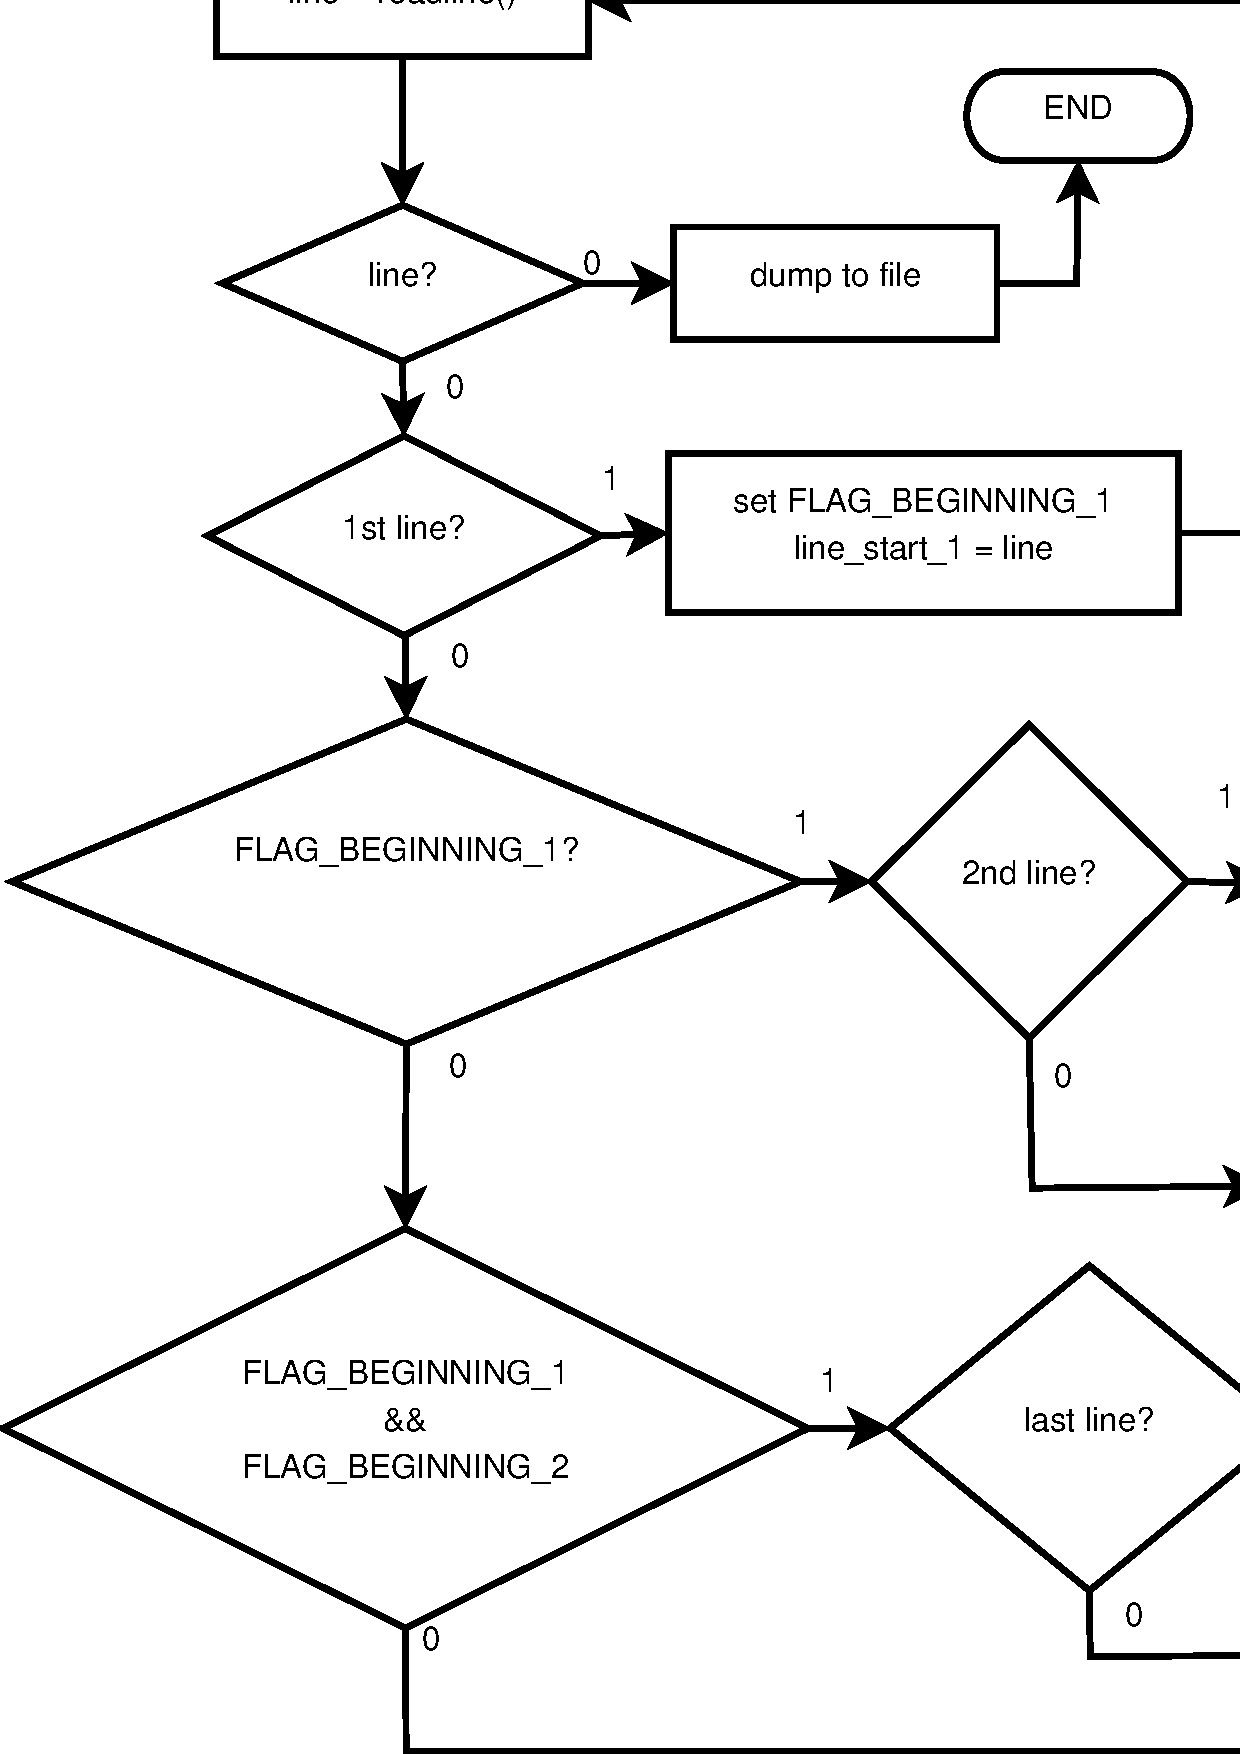
\includegraphics[width=0.98\textwidth]{./obrazky/TLE.pdf}
    \caption{Vývojový diagram extrahování dat TLE}
    \label{fig:TLE_flow}
  \end{figure}

\section{Korekce dopplerovského posuvu}
% gpredict -- libgpredict, doppler
% mediainfo, sox
  Po úspěšném získání nutných souborů s daty TLE pro umělé družice našeho zájmu, můžeme přistoupit ke korekci dopplerovského posuvu signálu, kterou provedeme pomocí programu doppler volně dostupného z repozitáře GIT týmu codehub dostupného na URL <\url{https://github.com/cubehub}>.

  Program doppler je utlitou příkazového řádku, který ze standardního vstupu čte IQ (in-phase, quadrature) data a zpracovává dle zadaných parametrů. Rozlišujeme dva režimy korekce frekvenčního posuvu. V režimu \emph{const} se kompenzuje konstantní posuv kmitočtu, kým v režimu \emph{track} se provádí korekce sledováním pohybu umělé družice a to i dodatečně v případě zpracování předem zaznamenaných dat IQ. V pozdním případě se programu doppler musí předát argument datu a času záznamu ve formátu ISO 8601 \cite{wiki:timeISO} \cite{github:doppler} bez udání časového posuvu v čase UTC.

  Korekce dopplerovského posuvu se provádí programem doppler za pomoci volně dostupné knihovny libgpredict, který je založen na predikčním kódu programu Gpredict. \cite{github:libgpredict}

  Aby se zjednodušilo zpracování velikého množství souborů, byl vytvořen skript v jazyce Python 3 pro automatické zpracování záznamů s IQ daty. Modul get\_undopplred má definovanou funkci undoppler\_it, který jako vstupní parametry má:
  \begin{itemize}
    \item název souboru IQ dat
    \item název družice v notaci OSCAR\footnote{v našém případě se jedná o NO-83, NO-84}
    \item kmitočet na kterém je z družice vysíláno
    \item adresář s IQ daty
    \item adresář s TLE daty
    \item lokace pozemní stanice
  \end{itemize}

  Pomocí těchto údajů se sestrojí řetězec obsahující příkaz shellu BASH, kde jednotlivé příkazy jsou řazeny do tzv. kolony. Jde o zřetězení příkazů oddělených metaznakem svislá čára '|'. Standardní výstup příkazu se předává standardnímu příkazu následujícímu. \cite{book:Brandejs-unix-linux}

  Parametry záznamu IQ dat se zjišťují pomocí modulu pymediainfo, který je tzv. wrapper function knihovny Mediainfo \cite{github:pymediainfo}. Pomocí tohoto modelu lze zjistit kmitočet vzorkování, bitovou hloubku, kódování, počet kanálů, kodek.

  Aby jsme mohli soubory formátu \zkratka{WAV} použít jako vstupní data pro program doppler, je nutné provést změnu formátu dle očekávání programu. K této úloze se použije volný program \zkratka{sox}. Podobně na výstupu lze použít \zkratka{sox} pro převod z RAW Audio formátu na \zkratka{WAV}.

  \begin{figure}[ht]
    \centering
    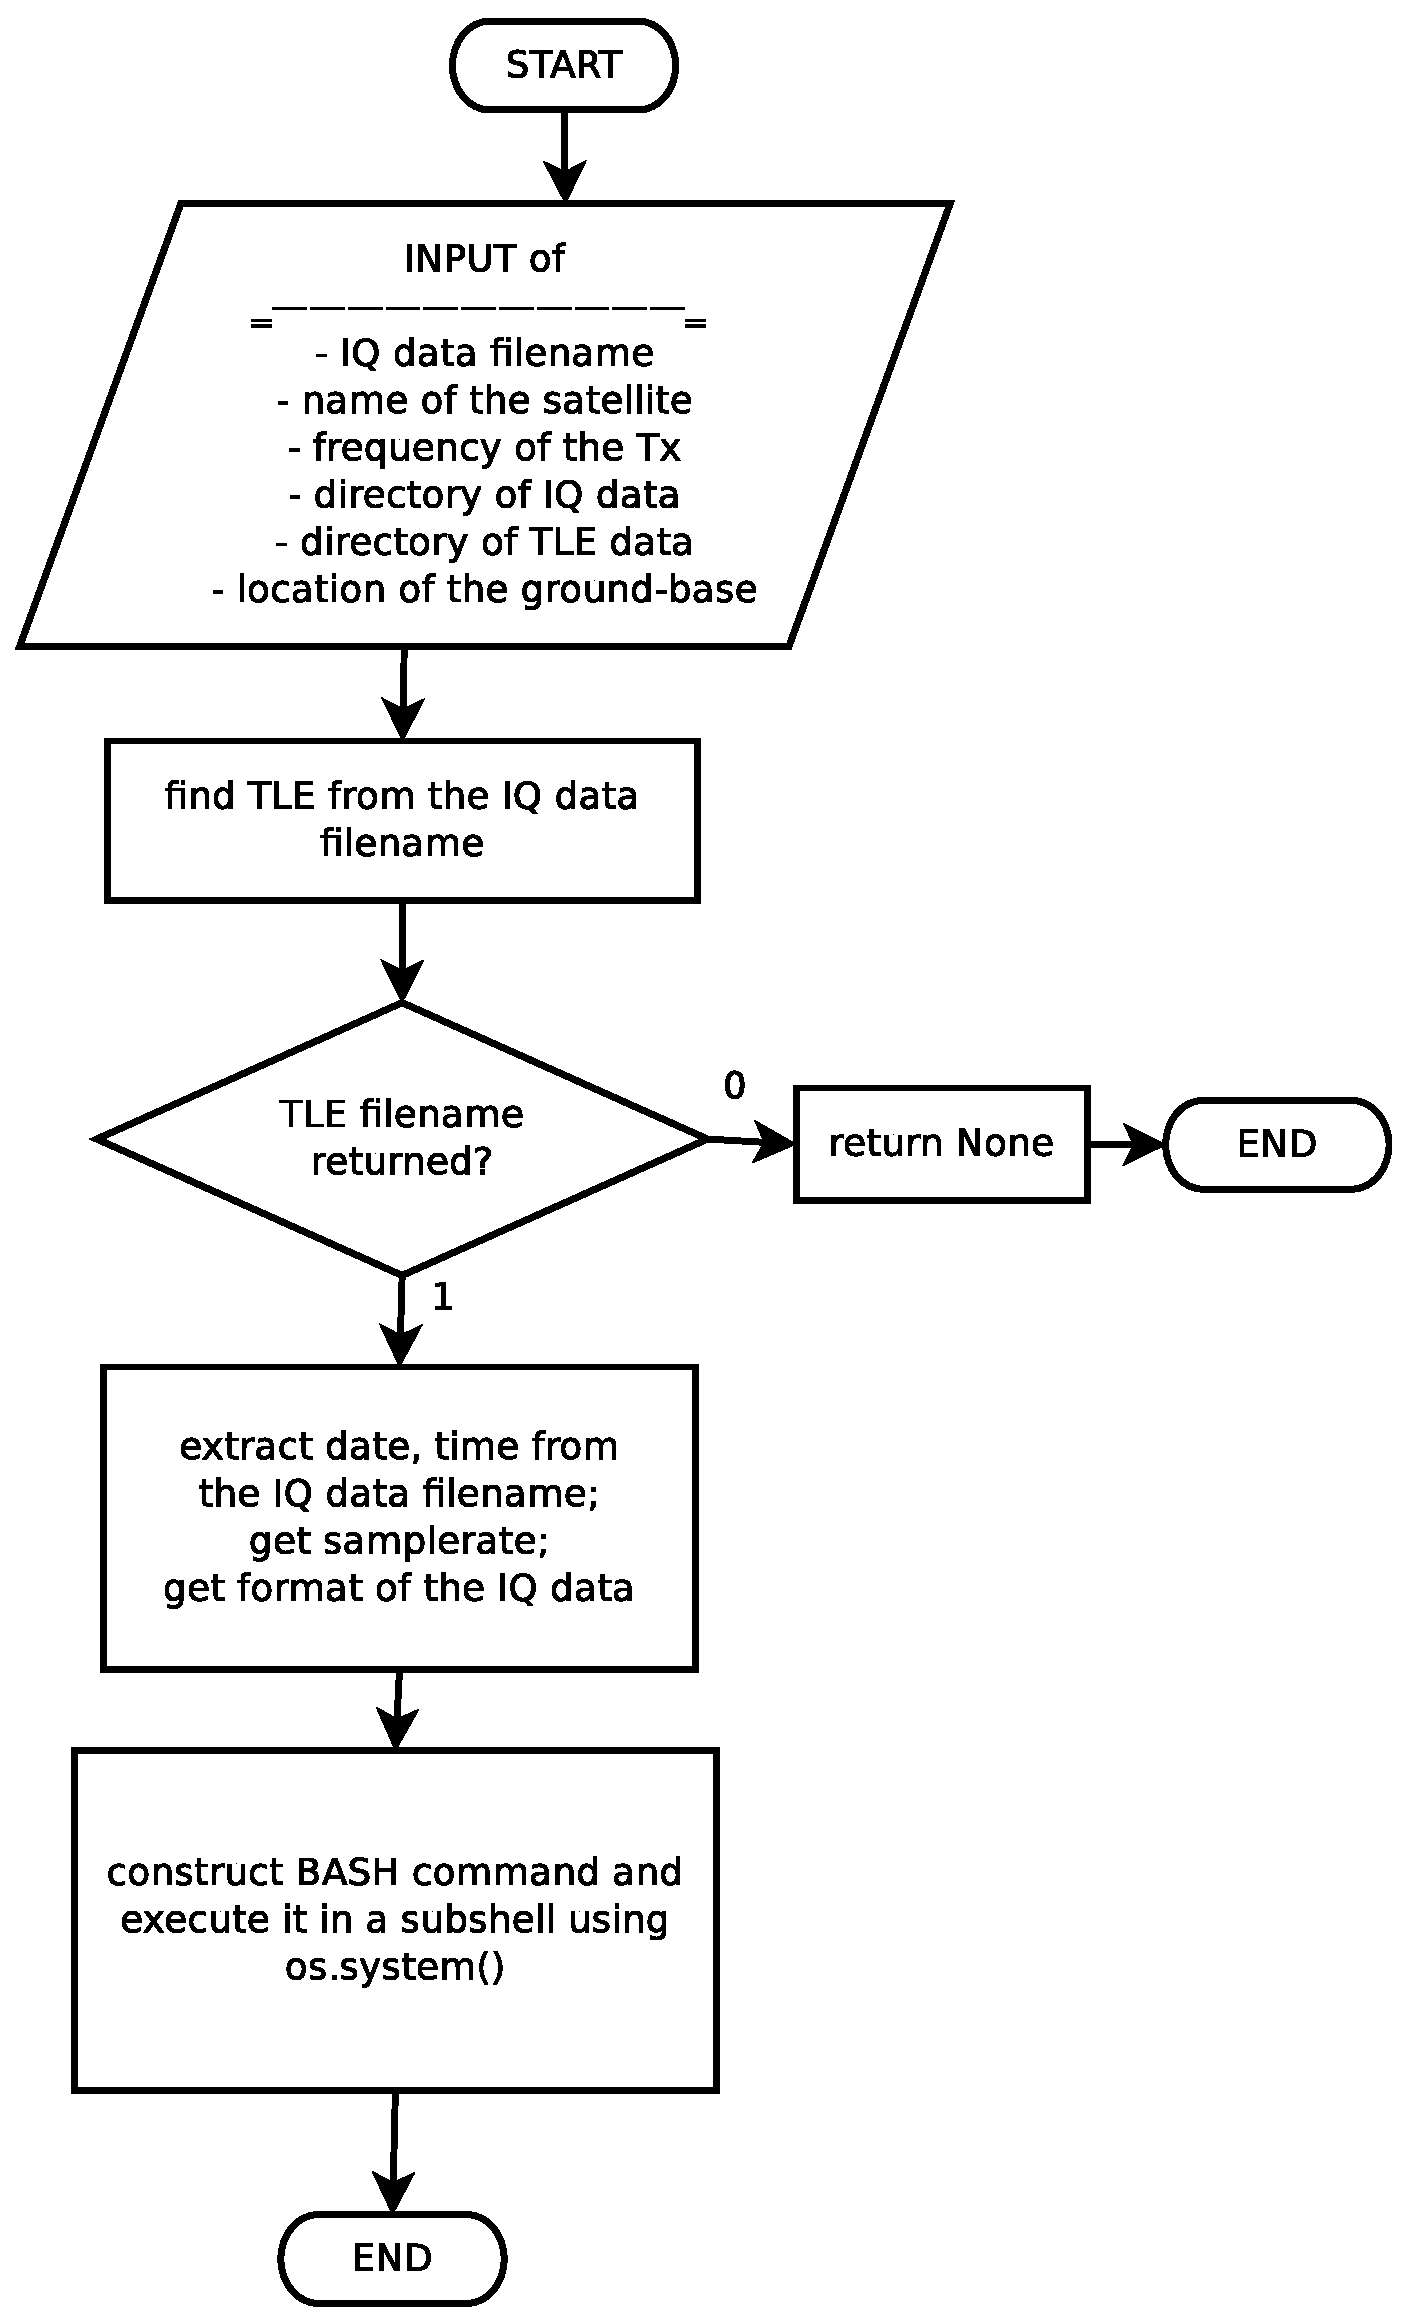
\includegraphics[width=0.65\textwidth]{./obrazky/get_undopplered.eps}
    \caption{Náčrt fungování modulu pro korekci dopplerovho posuvu}
    \label{fig:undoppler}
  \end{figure}

\section{Tvorba spektrogramů}

Kontrola správnosti korekci dopplerovského posuvu lze hrubě odhadnout pomocí spektrogramu korigovaných IQ dat. Pro automatizovaní tohoto procesu slouží modul wav2spectrogram.

Hlavní částí tohoto modulu je funkce IQ\_to\_spectrogram.
Python 3 modul pro tvorbu spektrogramů. Jediným argumentem je název souboru IQ dat. Ostatní parametry jsou buď napevno dány, nebo automaticky zjištění ze souboru IQ dat. Spektrogram je uložen ve formátu \zkratka{PNG}.

\section{Quo vadis moduly?}

Kudy směrují tyto moduly? Je filozofická otázka, na kterou by se dalo napsat nespočetné množství stran. Lze říct, že sami o sobě tyto moduly, skripty, neprovádějí automatické zpracování signálů, avšak jako základ pro budoucí vývoj mohou být nápomocné pro svou vlastnost zjednodušeného volání jinou funkcí, skriptem. Jazyk Python umožňuje jednoduchou iteraci nad všemi soubory složky, což nám dává možnost dávkového zpracování souborů s IQ daty.

Do budoucna se počítá s dalším zpracováním frekvenčně zkorigovaných signálů -- demodulace FM a následné dekódování přijatých zpráv telemetrie PSK31.


\chapter{Prezentace výsledků}
\label{chap:prez}

Funkčnost skript bylo ověřeno na záznamech signálů umělých družic NO-83, a NO-84.

Na obrázku \ref{fig:NO-84_raw} je znázorněn spektrogram přijatého rádiového signálu umělé družice NO-84. Dopplerův efekt lze zpozorovat na základě zjevného klesání kmitočtu přijatého signálu v závislosti na čase. Za předpokladu konstantního kmitočtu nosné vysílače a kmitočtu lokálního oscilátoru směšovače radiového přijímače můžeme usoudit, že umělá družice se k nám přibližuje a její relatívní rychlost vzhledem ke místu příjmu se zmenšuje.

Po aplikování korekci dopplerovského posuvu je spektrogram signálu znázorněn na obrázku \ref{fig:NO-84_ud}. Vidno, že drift kmitočtu od ideálního stavu přímky je minimální. Tyto odchylky jsou dány:

\begin{itemize}
  \item nepřesnost lokálního oscilátoru družice
  \item korekce kmitočtového posuvu po částech signálu diskrétní časové délky
  \item nepřesnost modelu SGP4 při předvídání pohybu družice
\end{itemize}

\begin{figure}[ht]
  \centering
  \includegraphics[width=0.9\textwidth]{./obrazky/HDSDR_20160123_152139Z_435320kHz_RF.png}
  \caption{Spektrogram signálu družice NO-84 bez korekce}
  \label{fig:NO-84_raw}
\end{figure}

\begin{figure}[ht]
  \centering
  \includegraphics[width=0.9\textwidth]{./obrazky/HDSDR_20160123_152139Z_435320kHz_RFUD.png}
  \caption{Spektrogram signálu družice NO-84 s korekcí}
  \label{fig:NO-84_ud}
\end{figure}

\begin{figure}[ht]
  \centering
  \includegraphics[width=0.9\textwidth]{./obrazky/HDSDR_20160127_161858Z_435320kHz_RF.png}
  \caption{Spektrogram signálu družice NO-83 bez korekce}
  \label{fig:NO-83_raw}
\end{figure}

\begin{figure}[ht]
  \centering
  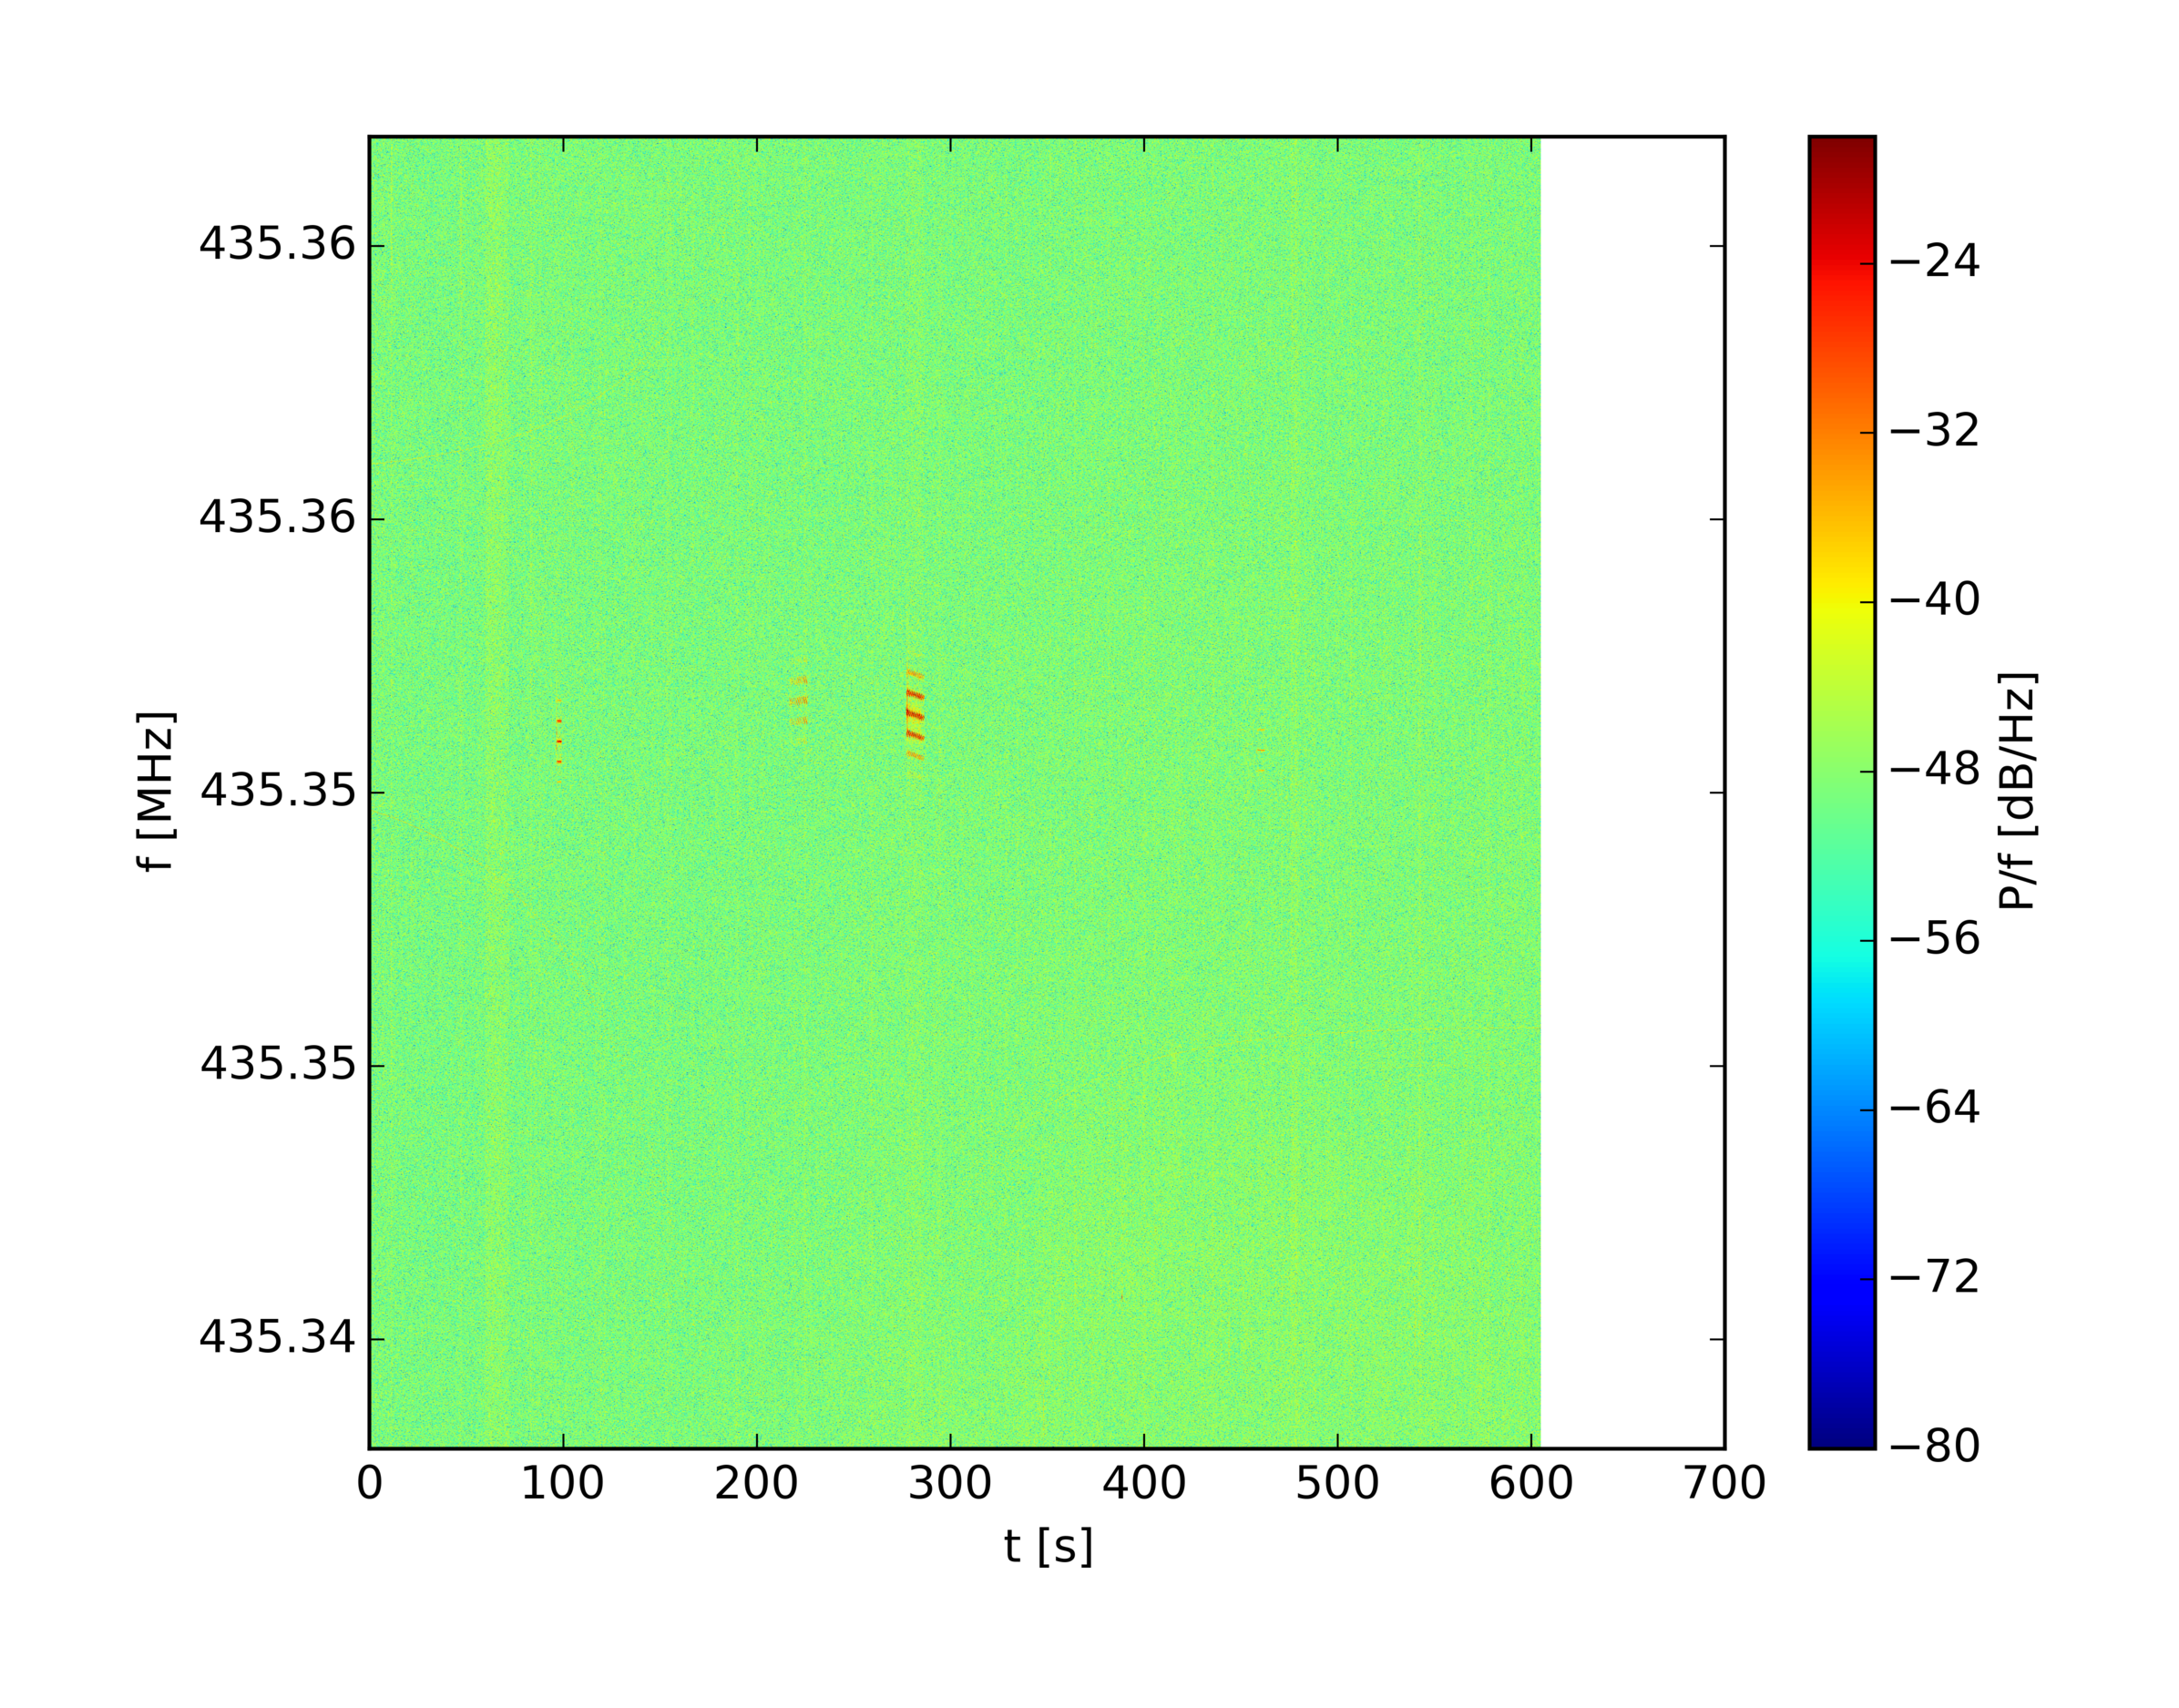
\includegraphics[width=0.9\textwidth]{./obrazky/HDSDR_20160127_161858Z_435320kHz_RFUD.png}
  \caption{Spektrogram signálu družice NO-83 s korekcí}
  \label{fig:NO-83_ud}
\end{figure}

  \chapter{Závěr}

Dopplerův jev je součástí našeho každodenního života, a to nejen v případě když vedle nás na železniční projede vysokorychlostní vlaková souprava dávající kontinuální výstražní signál, ale i v případě, že na ni sedíme a snažíme se naším mobilním komunikačním prostředkem provést datovou komunikaci prostřednictvím radiových signálů, avšak musí se poznamenat, že i rychlost nejrychlejšího vlaku je zanedbatelná vzhledem ke rychlosti družice na nízké oběžné dráze\footnote{viz. tabulka \ref{tab:orbit_vel}, najrýchlejši vlak pro osobní dopravu dle wikipedie dosahuje rychlosti $603\,\nicefrac{\mathrm{km}}{\mathrm{s}} = 0{,}1675\,\nicefrac{\mathrm{m}}{\mathrm{s}}$\cite{wiki:train}}.
Nejenom vysoká rychlost pohybu umělé družice, ale i použitý kmitočet z pásma $70\,\mathrm{cm}$ vln nás vede ke nutnosti korigování vzniklého dopplerovského posuvu kmitočtu signálu.

Táto část zadáni byla provedená bez jakýkoli zjištěné chyby. Jako ukazují spektrogramy v kapitole \ref{chap:prez} (obrázky \ref{fig:NO-84_raw} až \ref{fig:NO-83_ud}), korekce dopplerovského posuvu je do značné míry úspěšně provedeno. Cesta vývoje telemetrického archivu však žádném případě tady nekončí, a před námi je ještě několik problémů, které se musí zdolat.

Pokračováním projektu je demodulace a vytvoření databáze. Obdobně jako dosavadní práci, i další části projektu jsou plánovány být implementovány pomocí volného softwaru jako GNU Radio a SQLite, který pod licencí public domain \cite{{wiki:sqlite}}.

  % Pro sazbu seznamu literatury použijte jednu z následujících možností

%%%%%%%%%%%%%%%%%%%%%%%%%%%%%%%%%%%%%%%%%%%%%%%%%%%%%%%%%%%%%%%%%%%%%%%%%
%1) Seznam citací definovaný přímo pomocí prostředí literatura / thebibliography

\begin{literatura}{99}

\bibitem{wiki:amateur_sat}
    \emph{Amateur radio satellite}. In: Wikipedia: the free encyclopedia\/ [online].
    San Francisco (CA): Wikimedia Foundation, 2001- [cit. 2017-12-10].
    Dostupné z~URL:\\
    <\url{https://en.wikipedia.org/wiki/Amateur_radio_satellite}>.

\bibitem{wiki:AMSAT}
    \emph{Amateur radio satellite}. In: Wikipedia: the free encyclopedia\/ [online].
    San Francisco (CA): Wikimedia Foundation, 2001- [cit. 2017-12-10].
    Dostupné z~URL:\\
    <\url{https://en.wikipedia.org/wiki/AMSAT}>.

\bibitem{book:ARRL_handbook}
    PUBLISHED BY AMERICAN RADIO RELAY LEAGUE.
    \emph{The ARRL handbook for radio communications 2011.} 88th ed. Newington, CT: American Radio Relay League, 2010. ISBN 9780872590953.

\bibitem{wiki:LEO}
    \emph{Low Earth orbit}. In: Wikipedia: the free encyclopedia\/ [online].
    San Francisco (CA): Wikimedia Foundation, 2001- [cit. 2017-12-10].
    Dostupné z~URL:\\
    <\url{https://en.wikipedia.org/wiki/Low_Earth_orbit}>.

\bibitem{wiki:derbis}
    \emph{Space derbis}. In: Wikipedia: the free encyclopedia\/ [online].
    Dostupné z~URL:\\
    <\url{https://en.wikipedia.org/wiki/Space_debris}>.

\bibitem{wiki:US_space_surv}
    \emph{United States Space Surveillance Network}. In: Wikipedia: the free encyclopedia\/ [online].
    Dostupné z~URL:\\
    <\url{https://en.wikipedia.org/wiki/United_States_Space_Surveillance_Network}>.

\bibitem{wiki:TLE}
    \emph{Two-line element set}. In: Wikipedia: the free encyclopedia\/ [online].
    Dostupné z~URL:\\
    <\url{https://en.wikipedia.org/wiki/Two-line_element_set}>.

\bibitem{wiki:timeISO}
    \emph{ISO 8601}. In: Wikipedia: the free encyclopedia\/ [online].
    Dostupné z~URL:\\
    <\url{https://en.wikipedia.org/wiki/ISO_8601}>.

\bibitem{github:doppler}
    \emph{Doppler documentation}. [online].
    Dostupné z~URL:\\
    <\url{https://github.com/cubehub/doppler}>.

\bibitem{github:libgpredict}
    \emph{Libgpredict documentation}. [online].
    Dostupné z~URL:\\
    <\url{https://github.com/cubehub/libgpredict}>.

\bibitem{book:Brandejs-unix-linux}
    BRANDEJS, Michal.
    \emph{UNIX - Linux: praktický průvodce.} Praha: Grada, 1996. ISBN 80-7169-170-4.

\bibitem{github:pymediainfo}
    \emph{Pymediainfo github repository}. [online].
    Dostupné z~URL:\\
    <\url{https://github.com/sbraz/pymediainfo}>.

\bibitem{book:doppler_compensation}
    Gerorge P. Ah-Thew
    \emph{Doppler compensation for LEO satellite communication systems}. [online]
    <\url{https://macsphere.mcmaster.ca/bitstream/11375/5713/1/fulltext.pdf}>.

%\bibitem{\cite{wiki:orb_speed}
%    \emph{Orbital speed}. In: Wikipedia: the free encyclopedia\/ [online].
%    Dostupné z~URL:\\
%    <\url{https://en.wikipedia.org/wiki/Orbital_speed}>.
\bibitem{wiki:orb_speed}
    \emph{Orbital speed}. In: Wikipedia: the free encyclopedia\/ [online].
    Dostupné z~URL:\\
    <\url{https://en.wikipedia.org/wiki/Orbital_speed}>.

\bibitem{wiki:doppler_effect}
    \emph{Orbital speed}. In: Wikipedia: the free encyclopedia\/ [online].
    Dostupné z~URL:\\
    <\url{https://en.wikipedia.org/wiki/Doppler_effect}>.

\bibitem{wiki:train}
    \emph{Land speed record for rail vehicles}. In: Wikipedia: the free encyclopedia\/ [online].
    Dostupné z~URL:\\
    <\url{https://en.wikipedia.org/wiki/Land_speed_record_for_rail_vehicles}>.

\bibitem{wiki:sqlite}
    \emph{SQLite}. In: Wikipedia: the free encyclopedia\/ [online].
    Dostupné z~URL:\\
    <\url{https://en.wikipedia.org/wiki/SQLite}>.

%\bibitem{CSN_ISO_690-2011}
%    \emph{ČSN ISO 690 (01 0197) Informace a dokumentace -- Pravidla pro bibliografické odkazy a citace informačních zdrojů.}
%    40 stran. Praha: Český normalizační institut, 2011.
%
%\bibitem{CSN_ISO_7144-1997}
%    \emph{ČSN ISO 7144 (010161) Dokumentace -- Formální úprava disertací a podobných dokumentů.}
%    24 stran. Praha: Český normalizační institut, 1997.
%
%\bibitem{CSN_ISO_31-11}
%    \emph{ČSN ISO 31-11 Veličiny a jednotky -- část 11: Matematické znaky a značky používané ve fyzikálních vědách a v~technice.}
%    Praha: Český normalizační institut, 1999.
%
%\bibitem{BiernatovaSkupa2011:CSNISO690komentar}
%    BIERNÁTOVÁ, O., SKŮPA, J.:
%    \emph{Bibliografické odkazy a citace dokumentů dle ČSN ISO 690 (01 0197) platné od 1.\,dubna 2011}\/ [online].
%    2011, poslední aktualizace 2.\,9.\,2011 [cit. 19.\,10.\,2011].
%    Dostupné z~URL:
%    \(<\)\url{http://www.citace.com/CSN-ISO-690.pdf}\(>\)
%%    \(<\)\href{http://www.boldis.cz/citace/citace.html}{http://www.boldis.cz/citace/citace.html}\(>\).
%
%\bibitem{pravidla}
%    \emph{Pravidla českého pravopisu}.
%    Zpracoval kolektiv autorů. 1.\ vydání.
%    Olomouc: FIN PUB\-LISH\-ING, 1998. 575 s. ISBN 80-86002-40-3.
%
%\bibitem{Walter1999}
%  WALTER, G.\,G.; SHEN, X.
%  \emph{Wavelets and Other Orthogonal Systems}.
%  2. vyd. Boca Raton: Chapman\,\&\,Hall/CRC, 2000. 392~s. ISBN 1-58488-227-1
%
%\bibitem{Svacina1999IEEE}
%  SVAČINA, J.
%  Dispersion Characteristics of Multilayered Slotlines -- a Simple Approach.
%  \emph{IEEE Transactions on Microwave Theory and Techniques},
%  1999, vol.\,47, no.\,9, s.\,1826--1829. ISSN 0018-9480.
%
%\bibitem{RajmicSysel2002}
%    RAJMIC, P.; SYSEL, P.
%    Wavelet Spectrum Thresholding Rules.
%    In \emph{Proceedings of the International Conference Research in Telecommunication Technology},
%    Žilina: Žilina University, 2002. s.\,60--63. ISBN 80-7100-991-1.

\end{literatura}


%%%%%%%%%%%%%%%%%%%%%%%%%%%%%%%%%%%%%%%%%%%%%%%%%%%%%%%%%%%%%%%%%%%%%%%%%
%%2) Seznam citací pomocí BibTeXu
%% Při použití je nutné v TeXnicCenter ve výstupním profilu aktivovat spouštění BibTeXu po překladu.
%% Definice stylu seznamu
%\bibliographystyle{unsrturl}
%% Pro českou sazbu lze použít styl czechiso.bst ze stránek
%% http://www.fit.vutbr.cz/~martinek/latex/czechiso.tar.gz
%%\bibliographystyle{czechiso}
%% Vložení souboru se seznamem citací
%\bibliography{text/literatura}
%
%% Následující příkaz je pouze pro ukázku sazby literatury při použití BibTeXu.
%% Způsobí citaci všech zdrojů v souboru odkazy.bib, i když nejsou citovány v textu.
%\nocite{*}

  \begin{seznamzkratek}{KolikMista}

  \novazkratka{AMSAT}                        % název
      {AMSAT-NA}                             % zkratka
      {Radio Amateur Satellite Corporation}  % rozvinutí zkratky

  \novazkratka{OSCAR}
      {OSCAR}
      {Orbiting Satellite Carrying Amateur Radio}

  \novazkratka{USSTRATCOM}
      {USSTRATCOM}
      {United States Strategic Command}

  \novazkratka{DoD}
      {DoD}
      {Department of Defense}

  \novazkratka{ESA}
      {ESA}
      {European Space Agency}

  \novazkratka{Fraunhofer-FHR}
      {Fraunhofer-FHR}
      {Fraunhofer-Institut fur Hochfrequenzphysik und Radartechnik}

  \novazkratka{TIRA}
      {TIRA}
      {Tracking \& Imaging Radar}

  \novazkratka{NASA}
      {NASA}
      {National Aeronautics and Space Administration}

  \novazkratka{JPL}
      {JPL}
      {Jet Propulsion Laboratory}

  \novazkratka{GDSCC}
      {GDSCC}
      {Goldstone Deep Space Communications Complex}

  \novazkratka{MIT}
      {MIT}
      {Massachusetts Institute of Technology}

  \novazkratka{EISCAT}
      {EISCAT}
      {European Incoherent Scatter Scientific Association}

  \novazkratka{USAF}
      {USAF}
      {United States Air Force}

  \novazkratka{TLE}
      {TLE}
      {two-line elements}

  \novazkratka{SGP4}
      {SGP4}
      {Simplified perturbations models}

  \novazkratka{UTC}
      {UTC}
      {Coordinated Universal Time}

  \novazkratka{WAV}
      {WAVE}
      {Waveform Audio File Format}

  \novazkratka{sox}
      {SoX}
      {Sound eXchange}

  \novazkratka{PNG}
      {PNG}
      {Portable Network Graphics}


%  %%% bsymfvz
%  \novazkratka{symfvz}            % název
%    {\ensuremath{f_\textind{vz}}} % symbol
%    {vzorkovací kmitočet}          % popis
%  %%% esymfvz

\end{seznamzkratek}


%%%%%%%%%%%%%%%%%%%%%%%%%%%%%%%%%%%%%%%%%%%%%%%%%%%%%%%%%%%%%%%%%%%%%%%%%%%%%%%%
% Csatolmányok
  \prilohy
  \seznampriloh
  \chapter{Zdrojové kódy}

  \section{Skript \texttt{TLE.py}}

    Python 3 modul pro extrahování TLE dat.
    \lstinputlisting[numbers=left, breaklines=true, language=Python]{/home/ptoth/Documents/Projekt/github/projekt17/Python3/TLE.py}

  \section{Skript \texttt{get\_undopplered.py}}

    Python 3 modul pro korekci dopplerovského posuvu.
    \lstinputlisting[numbers=left, breaklines=true, language=Python]{/home/ptoth/Documents/Projekt/github/projekt17/Python3/get_undopplered.py}

  \section{Skript \texttt{wav2spectrogram.py}}

    Python 3 modul pro tvorbu spectrogramů.
    \lstinputlisting[numbers=left, breaklines=true, language=Python]{/home/ptoth/Documents/Projekt/github/projekt17/Python3/wav2spectrogram.py}


\end{document}
